\documentclass[UTF8,a4paper]{ctexart}
\usepackage[margin=1in]{geometry}
\usepackage{fancyhdr,hyperref,amsmath,float,graphicx,color,float}
\pagestyle{fancy}
\hypersetup{hidelinks}

\lhead{\bfseries \leftmark}
\chead{}
\rhead{SCUT}
\lfoot{\url{https://github.com/285571052}}
\cfoot{qhy}
\rfoot{\thepage}
\setlength{\headheight}{13pt}
\renewcommand{\headrulewidth}{0.4pt}
\renewcommand{\footrulewidth}{0.4pt}

\setlength{\parindent}{0pt}
\newcommand{\spaceline}{\vspace{\baselineskip}}

\author{ qhy }
\date{\today}
\title{计算机网络}

\begin{document}
  \maketitle
  \tableofcontents
  \newpage

  \section{介绍}
  %2017-9-5:第一节课主要简单介绍的mac地址,ip以及协议相关内容。
  \textbf{WWW:}world wide web,是信息资源的网络,\textbf{资源}、 \textbf{资源标识} 、 \textbf{传输协议} 三部分支撑www的运转做。

  \textbf{拓扑}:信道的分布方式 , 常见的拓扑结构有: 总线型, 星型 , 环型 ,树型 , 网状

  \textbf{协议:}一系列规则和规定的规范性描述 ,它控制网络中的设备之间如何进行信息交换

  \textbf{数字带宽:} 指在单位时间内流经的信息总量,单位:bps , kbps , Mbps , Gbps(一般取$10^3$计算)

  \textbf{吞吐量}:指实际的、可观测到的带宽

  \textbf{传输时间:}
  $T = \frac{S}{BW} \quad T = \frac{S}{P}$

  \textbf{单位问题:}$1B = 8b , 1M = 1MB$(省略了的是$B$)

  \textbf{点到点:}两个机器的直接物理连接

  \textbf{端到端:}信源机 与 信宿机 之间的直接通信 , 好像拥有一条直接的线路

  网络分类:
  \begin{itemize}
    \item 按传输技术:广播式网络, 点到点网络
    \item 按传输距离:个域网(PAN,1m) , 局域网(LAN,10m-1km) , 城域网(MAN,10km) , 广域网(WAN, 10-1000km) , 互联网(Internet,10000km)
    \item 按传输介质:有线网 , 无线网
    \item 按拓扑结构: 总线 , 环型 , 网状 , 星型
  \end{itemize}

  \textbf{网关:}连接异构网络, 提供必要的转换

  \textbf{互连网络}:网络的集合 , 主要形式:被WAN连接起来

  \textbf{子网、网络、互联网}:子网完成基础转发 , 子网和主机组成网络

  \section{参考模型}

  \textbf{协议:}一系列规则和规定的规范性描述 ,它控制网络中的设备之间如何进行信息交换。

  网络协议的三个要素:
  \begin{itemize}
    \item 语法: 数据与控制信息的结构或格式
    \item 语义: 控制信息, 指出完成的动作及响应
    \item 同步: 事件执行顺序的详细说明
  \end{itemize}

  \subsection{分层模型}

  \textbf{协议分层的优点:}
  \begin{itemize}
    \item 各层工作独立, 层时间通过接口联系 , 降低协议工作的复杂程度
    \item 灵活性好 , 任何一层的改变不影响其他层
    \item 每层的实现技术可以不同 ,减少了实现的复杂度
    \item 易于维护 , 每层可以单独进行调试
    \item 便于标准化
  \end{itemize}

  \textbf{分层的意义:}
  \begin{itemize}
    \item 网络互连的自然需求
    \item 分而治之, 简化网络操作
    \item 提供即插即用的兼容性和不同厂商之间集成的标准
    \item 使工程师们可以专注于某一功能模块的设计和优化
    \item 防止不同区域网络之间的相互影响
  \end{itemize}

  \textbf{分层原则}:信宿机第n层收到的对象应与信源机第n层发出的对象完全一致

  \textbf{典型分层模型}:OSI七层模型 , TCP/IP(DoD)四层模型

  \textbf{每一层的功能:}为它的上一层服务

  \textbf{实体Entity}:每层中活动的元素

  \textbf{对等实体peer}

  \textbf{层与层 之间的关系}:第n层是服务提供者, 第n+1层是服务独享, 即服务的消费者(下方的层是低层)
  \begin{figure}[H]
    \centering
    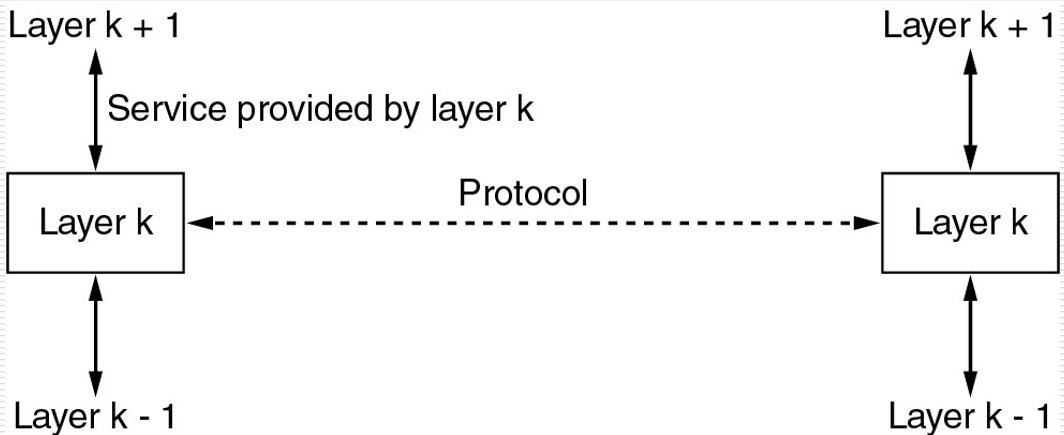
\includegraphics[scale = 0.3]{assets/jisuanjiwangluo_ce243.png}
    \caption{层和协议的关系}
  \end{figure}

  \textbf{协议数据单元}:PDU , protocol data unit

  \subsection{ISO-OSI模型}
  ISO-OSI模型:
  \begin{itemize}
    \item 协议很少再使用, 但模型却很流行
    \item 每层都定义了标准
    \item 本身不是网络架构,因为它本身并没有规定每层确切的服务和协议
  \end{itemize}
  \begin{figure}[H]
    \centering
    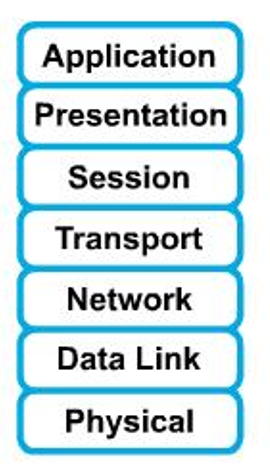
\includegraphics[scale = 0.3]{assets/jisuanjiwangluo_492ef.png}
    \caption{7层OSI模型}
  \end{figure}

  \begin{figure}[H]
    \centering
    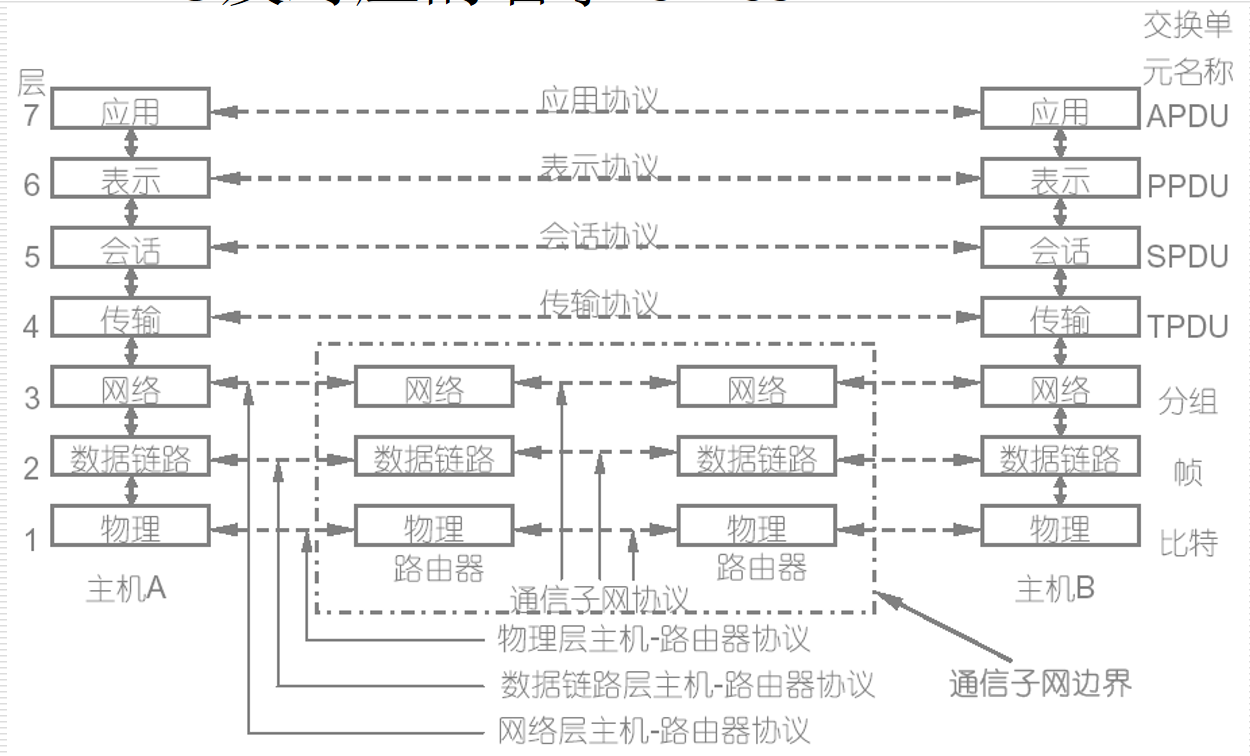
\includegraphics[scale = 0.3]{assets/jisuanjiwangluo_63c15.png}
    \caption{PDU及对应的名字}
  \end{figure}

  \begin{figure}[H]
    \centering
    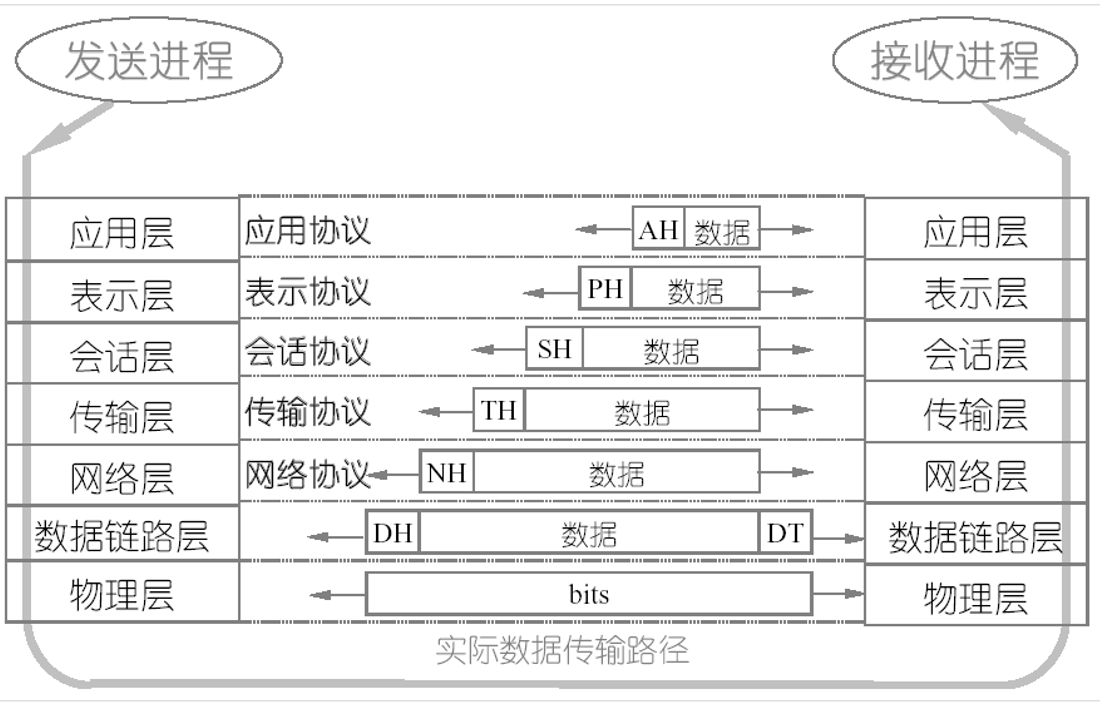
\includegraphics[scale = 0.3]{assets/jisuanjiwangluo_3ab21.png}
    \caption{OSI参考模型上的数据流}
  \end{figure}

  \begin{figure}[H]
    \centering
    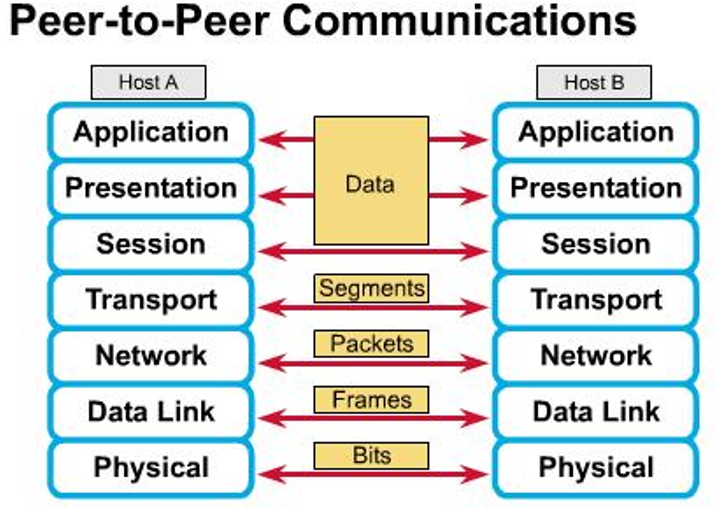
\includegraphics[scale = 0.3]{assets/jisuanjiwangluo_6d9c7.png}
    \caption{对等通信、虚拟通信}
  \end{figure}

  \textbf{为什么OSI参考模型没有占据主流?}糟糕的时机, 糟糕的技术 ,糟糕的实现 ,糟糕的政策
  \begin{itemize}
    \item 糟糕的时机\\
    当OSI协议出现的时候,与之竞争的TCP/IP协议已经被广泛地应用于大学和科研机构,没有厂家愿意支持第二个协议栈

    \item 糟糕的技术\\
    会话层和表示层几乎为空, 数据链路层和网络层包含太多的内容\\
    OSI模型以及相应的服务定义和协议都极其复杂,难以实现,操作起来也和低效
    \item 糟糕的实现\\
    OSI模型和协议过于复杂,最初的实现不仅庞大而且笨拙,效率也很慢
    \item 糟糕的政策\\
    政府官僚试图把技术不足的标准强加给那些实际开发计算机网络的可怜的研究人员和程序员
  \end{itemize}

  \subsection{TCP/IP参考模型}
  TCP/IP模型:
  \begin{figure}[H]
    \centering
    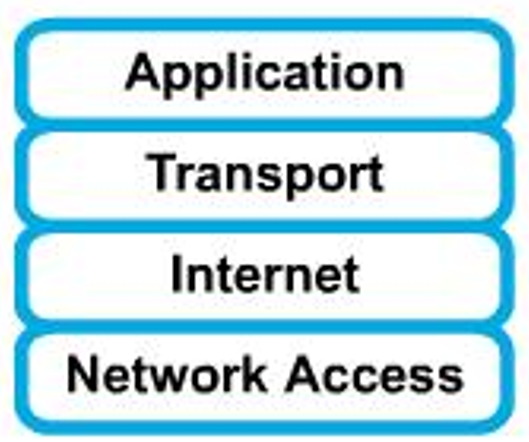
\includegraphics[scale = 0.3]{assets/jisuanjiwangluo_0c1c0.png}
    \caption{TCP/IP模型}
  \end{figure}

  \begin{itemize}
    \item 互联网层\\
  与OSI中的网络层对应\\
  该层定义了正式的分组格式和协议 , 即 IP协议 ,每个IP包的路由问题是由互联网\\
  每个IP包肚子寻径 , 到达顺序可能不相同
  \item 传输层\\
  与OSI中的传输层对应\\
  使源端和目的端主机的对等实体进行对话\\
  蒂尼了两个端到端的协议:TCP传输控制协议 , 用户数据报协议UDP
  \item 应用层\\
  与OSI中的上三层相对应\\
  该层包括:telnel标准终端仿真协议 , ftp文件传输协议 , smtp简单邮件传输协议 , 域名解析服务DNS
  \end{itemize}

  \begin{figure}[H]
    \centering
    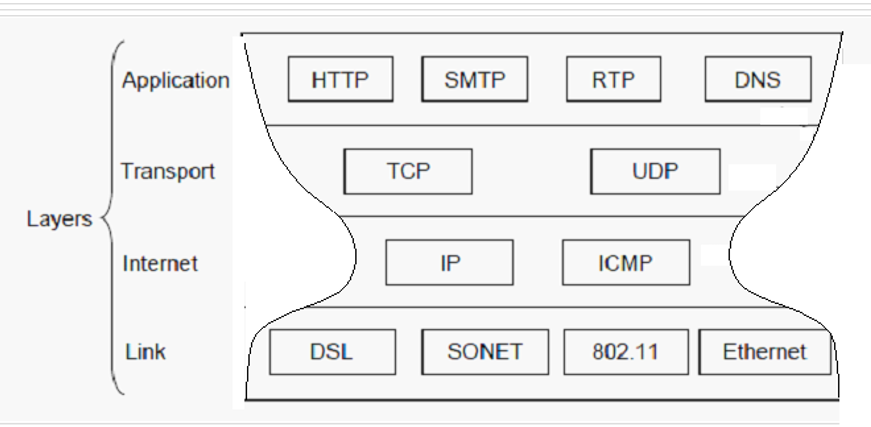
\includegraphics[scale = 0.3]{assets/jisuanjiwangluo_8c48b.png}
    \caption{TCP/IP参考模型中的协议}
  \end{figure}

  \textbf{TCP/IP参考模型和协议的缺点:}
  \begin{itemize}
    \item 没有区分服务、接口和协议的概念
    \item 不是通用的模型
    \item 主机至网络层不是常规意义上的层
    \item 没有区分物理层和数据链路层
    \item 有些协议的实现比较草率
  \end{itemize}

  TCP/IP参考模型和OSI模型的对比:
  \begin{figure}[H]
    \centering
    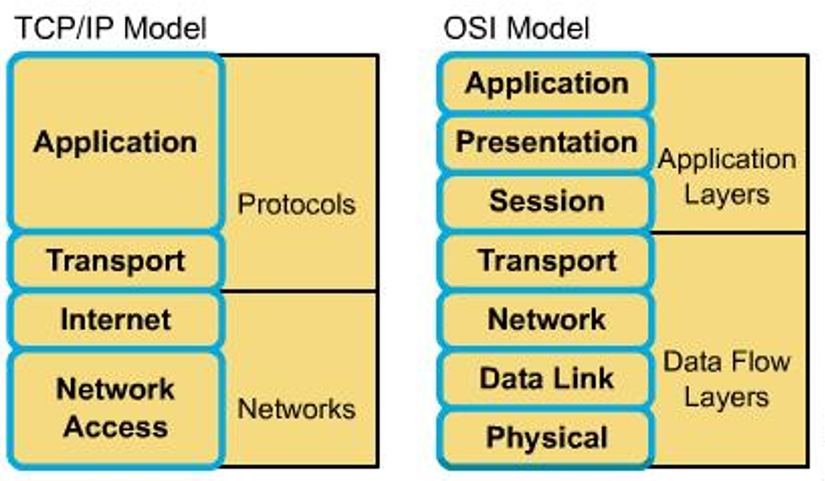
\includegraphics[scale = 0.3]{assets/jisuanjiwangluo_60bc3.png}
  \end{figure}

  相同点:
  \begin{itemize}
    \item 都分层
    \item 都有应用层,尽管他们提供的服务不同
    \item 使用的分组交换而不是电路交换技术
  \end{itemize}

  不同点:
  \begin{itemize}
    \item TCP/IP将 表示层 和 会话层 包含到了 应用层
    \item TCP/IP将OSI的数据链路层和物理层包括到了一层中
    \item TCP/IP更简洁, 但OSI更易开发和排除故障
    \item TCP/IP在实践中产生
  \end{itemize}

  \subsection{混合参考模型}
  计算机网络书中的参考模型:
  \begin{figure}[H]
    \centering
    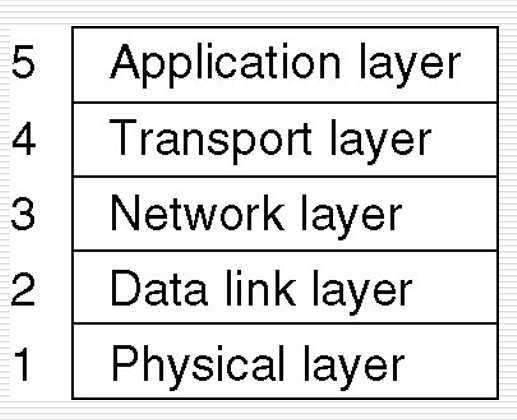
\includegraphics[scale = 0.3]{assets/jisuanjiwangluo_39666.png}
    \caption{混合参考模型}
  \end{figure}

  \section{物理层}
  物理层上信号的传输:信号

  有两类:模拟信号;数字信号

  \textbf{物理层的功能} :在两个网络设备之间提供透明的比特流传输

  \textbf{物理层的4个特性}:机械特性 ,电气特性, 功能特性,规程特性

  \subsection{傅里叶分析}
  傅里叶级数: 任何正常周期为T的函数g(t) , 都可由(无限个)正弦和余弦函数合成

  任何信号的传输都可理解为以傅里叶级数的形式传递

  \begin{figure}[H]
    \centering
    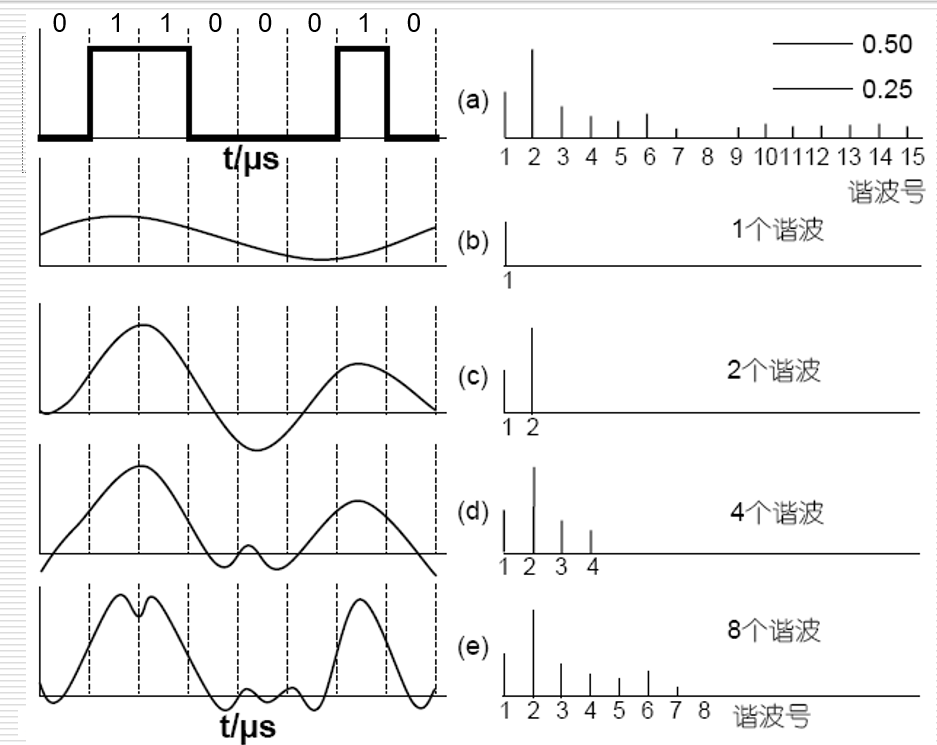
\includegraphics[scale = 0.3]{assets/jisuanjiwangluo_f186a.png}
    \caption{谐波数越高,传输质量越好}
  \end{figure}

  如果每个傅里叶级数的信号分量被等量衰减,则合成后,振幅有所衰减, 基本形状不变

  但,所有的传输设备对不同傅里叶分量的衰减并不相同 ,因此会导致信号变形( \textbf{失真})

  信号在传输的过程中,接收方接受到的信号可能是衰减和变形的(失真)

  一般来说, 从$0-f_c$这一频段, 振幅在传输过程不会明显衰减 ,则$f_c$称为 \textbf{截止频率}

  \textbf{(物理)带宽}:传输工程中振幅不会明显瞬间的频率范围,是一种 \textbf{物理特性},通常取决于介质的材料构成、厚度、长度等
  \footnote{\textbf{数字带宽:} 指在单位时间内流经的信息总量,单位:bps , kbps , Mbps , Gbps(一般取$10^3$计算)}
  \footnote{\textbf{吞吐量}:指实际的、可观测到的带宽}

  \textbf{物理带宽和数字带宽的关系是???????????????}

  \begin{figure}[H]
    \centering
    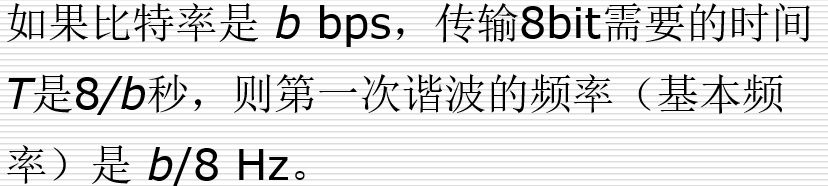
\includegraphics[scale = 0.3]{assets/jisuanjiwangluo_ee963.png}
    \caption{频率是时间的倒数}
  \end{figure}

  信道的最大数据传输速率:奈奎斯特定理(理想信道, 无噪声信道) , 香农定理(有噪声信道)
  \begin{itemize}
    \item 奈奎斯特 Nquist 定理\\
    在无噪声信道中, 当带宽为 $B hz$ , 信号电平为$V$级,则:\\
    最大传输速率为$2B \log_2 V bps$\\
    其中, $V$为信号的电平级数 , 在二进制中 ,一位表示0或1 , V级可以表示$\log_2 V$位,
    而对于带宽B最多有2B次采样
    \footnote{奈奎斯特定理:关于2B次的一个理解:假设一个正弦波, 采样点的值为正表示1 , 为负表示2 , 那么一个周期内最多能表示2个值 , 如果我们在一个周期内采样3次,那么必定有一次是无用的,即一个周期最多采样两次, 而已知频率为B , 那么采样的频率最大只能为 2B , 否则解析信号结果和想要发送的结果将不一致}
    \footnote{2B表示波特率}
    \item 香农 Shannon 定理\\
    在噪声信道中, 带宽为$B Hz$ , 信噪比为$\frac{S}{N}$ , 则 \\
    最大传输速率为: $B\log_2(1 + \frac{S}{N}) bps$\\
    很多时候,噪声使用 分贝 dB 表示:$10 \log_{10} \frac{S}{N} db$
    \footnote{香农定理:噪声为$1$, 信号为$\frac{S}{N}$}
  \end{itemize}

  \begin{figure}[H]
    \centering
    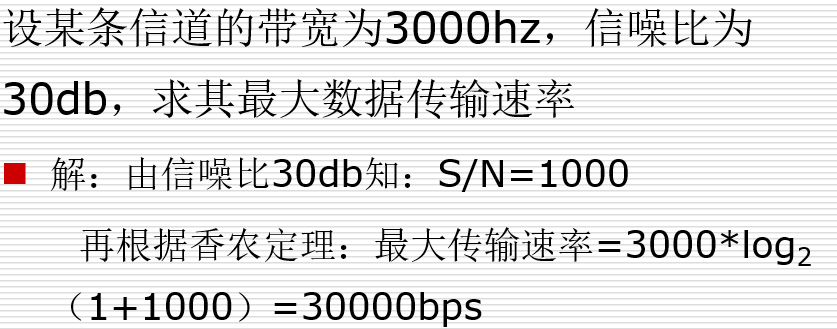
\includegraphics[scale = 0.3]{assets/jisuanjiwangluo_d4de4.png}
  \end{figure}

  \begin{figure}[H]
    \centering
    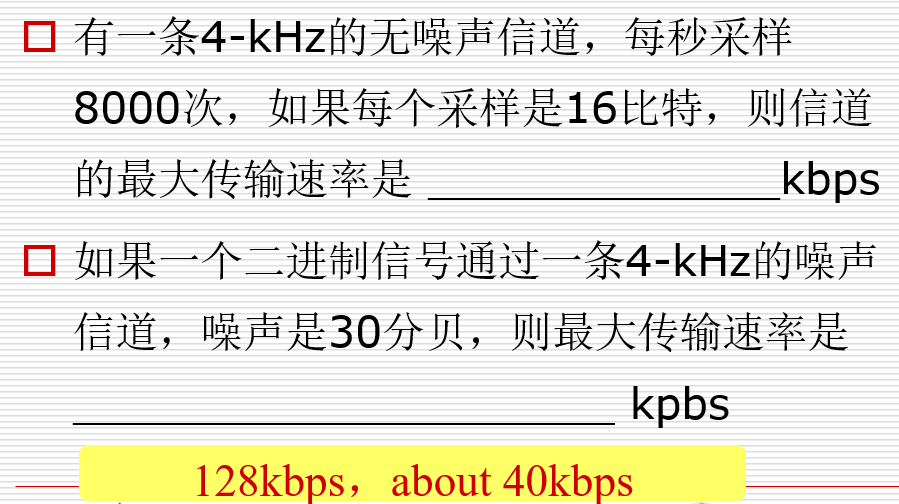
\includegraphics[scale = 0.3]{assets/jisuanjiwangluo_e6df3.png}
  \end{figure}

  \begin{figure}[H]
    \centering
    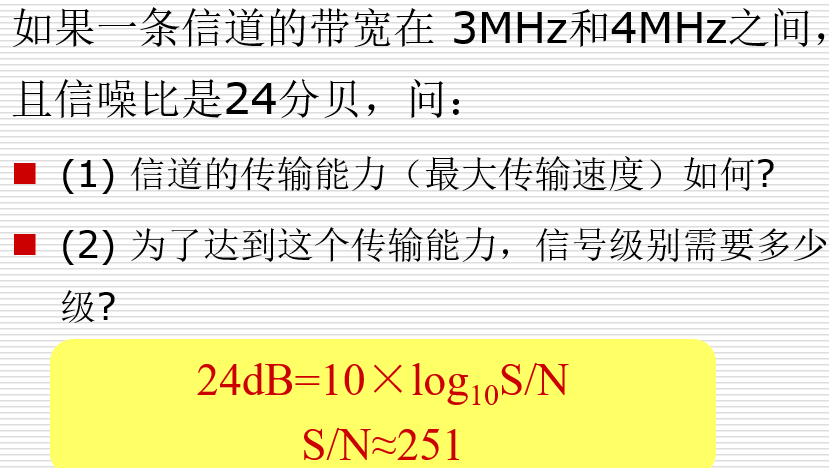
\includegraphics[scale = 0.3]{assets/jisuanjiwangluo_81802.png}
    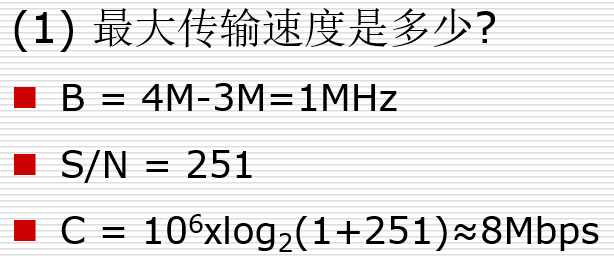
\includegraphics[scale = 0.3]{assets/jisuanjiwangluo_bef5b.png}
    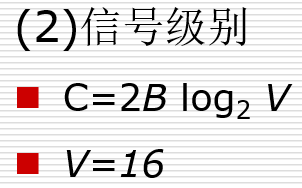
\includegraphics[scale = 0.3]{assets/jisuanjiwangluo_af2c8.png}
  \end{figure}

  \subsection{传输介质}
  \begin{itemize}
    \item 磁介质
    \begin{figure}[H]
      \centering
      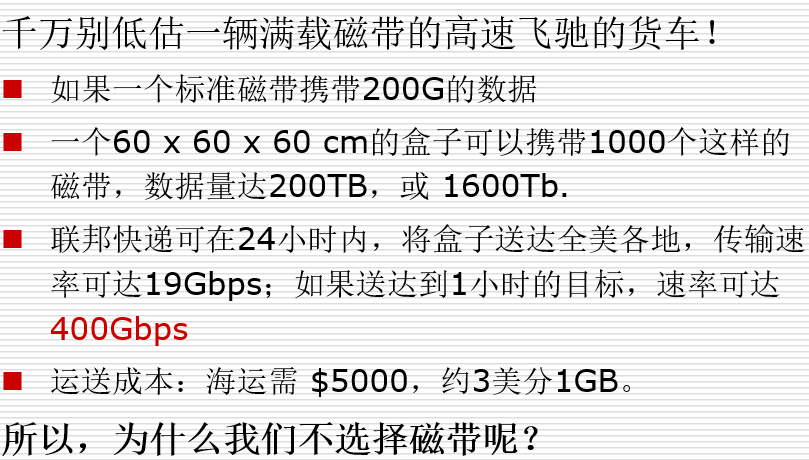
\includegraphics[scale = 0.3]{assets/jisuanjiwangluo_080be.png}
      \caption{有趣的例子}
    \end{figure}
    \item 双绞线:非屏蔽双绞线(UTP) , 屏蔽双绞线(STP)\\
    两个具有绝缘层的铜线按一定密度,逆时针方向绞合而成 , 一般绞距越小(紧),则抵消效果
    越好, 传输性能越好 \\
    非屏蔽:成本低;尺寸小;易于安装但易受干扰;传输距离性能受绞距影响;受绞距限制,功能有限,最大传输距离100m(短);10~100Mbps\\
    STP 屏蔽双绞线:4对线,每对线都有屏蔽层,最外面还有一层屏蔽层,成本高,安装不容易;最大距离100m,10~1000=Mbps\\
    网屏式双绞线,保留最外的屏蔽层,除了屏蔽性能,其他是一样的\\
    双绞线的线序:568B,568A(直通线,两根头的线序相同,交叉线,线序相反)
    \begin{figure}[H]
      \centering
      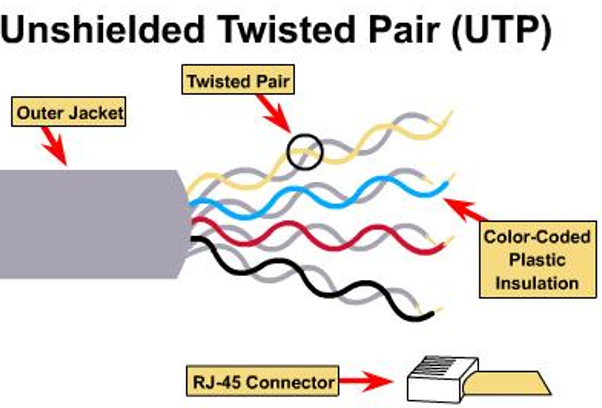
\includegraphics[scale = 0.3]{assets/jisuanjiwangluo_fa7df.png}
      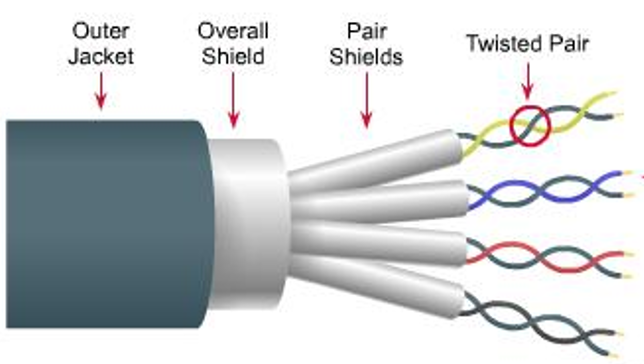
\includegraphics[scale = 0.3]{assets/jisuanjiwangluo_70eb1.png}
      \caption{双绞线}
    \end{figure}
    \item 同轴电缆:由中心导体;绝缘层;网状导体;外部绝缘层组成
    \begin{figure}[H]
      \centering
      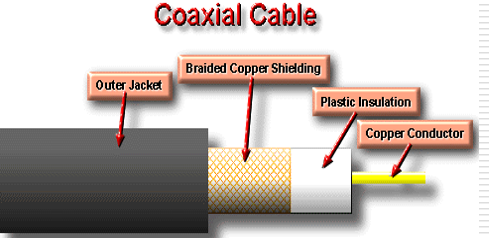
\includegraphics[scale = 0.3]{assets/jisuanjiwangluo_68b5a.png}
      \caption{同轴电缆}
    \end{figure}
    粗缆:最大传输距离500m,两端安装终接器,以保证电缆屏蔽层接地\\
    细缆:最大传输距离185m,两头安装BNC头,接在T型连接器两端
    \item 电力线
    \item 光纤(光导纤维):由极细的玻璃纤维构成,把光封闭在其中并沿轴向进行传播\\
    3层,两层玻璃纤维,最外层为防护层\\
    原理:全反射,因而损耗低\\
    优点:重量轻;损耗低;不收电磁辐射干扰;传输频带,通信容量大\\
    缺点:昂贵;易断裂\\
    单模光纤:以单一模式传输,激光产生单束光(8-10 um) , 纤芯细 , 高带宽,长距离,运行波长为850nm或1300nm\\
    多模光纤:以多个模式(多个入射角 , 只要大于临界角度)同时传输,LED产生的多束光 , 纤芯粗(50-62.5um) ,低带宽, 短距离,运行波长为1310或1550nm
    \begin{figure}[H]
      \centering
      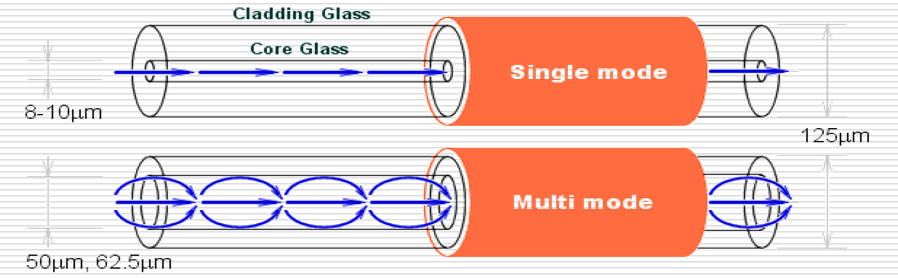
\includegraphics[scale = 0.3]{assets/jisuanjiwangluo_4ce0a.png}
    \end{figure}
    光纤连接:光纤连接器(光损失10\%-20\%) ; 机械拼接,特殊的套管夹紧(光损失10\%);熔合(几乎无损失)\\
    光纤比铜线的特性:带宽高;距离远;耗损低;重量轻;无电磁干扰和射频干扰;防窃听;端口设备价格高
  \end{itemize}

  \subsection{数字调制和复用}

  \spaceline
  $\left \{ \begin{array}{l}
  \text{基带传输:直接将数据比特转换成信号,使用高低调位为标准描述0/1两个信号}\\
  \text{通带传输:通过调节信号的振幅;相位;频率来传输比特,使用振幅,频率,相位等为标准描述}
  \end{array} \right .$

  \subsubsection{基带传输}

  \begin{figure}[H]
    \centering
    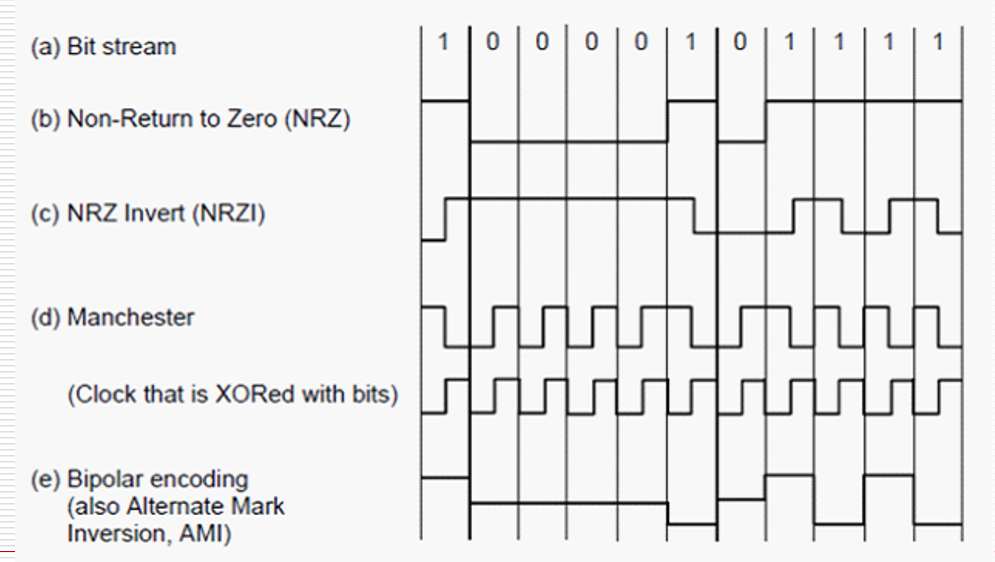
\includegraphics[scale = 0.3]{assets/jisuanjiwangluo_cc3d9.png}
    \caption{基带传输}
  \end{figure}
  \begin{itemize}
    \item [(b)] NRZ:高电平表示1,低电平表示0
    \item [(c)] 不归0逆转;NRZ Invert;NRZI:跳变表示1 , 不变表示0
    \item [(d)] Mncheter:高跳变到低表示1 ,低跳变到高表示0
    \item [(e)] 双极性编码:0始终用一个中间电压表示,1使用高电压表示之后使用低电压表示,中间表示0 ,两边表示1 , 连续1 跳变
  \end{itemize}

  \textbf{波特率(符号率;采样率):}每秒信号变化的次数。

  \textbf{比特率(位传输率;数据传输率)与波特率的关系}:
  \[C = B \times \log_2 n\]
  其中,C为比特率, B为波特率, n为电平数 或 线路的状态数

  \subsubsection{通带传输}
  \begin{figure}[H]
    \centering
    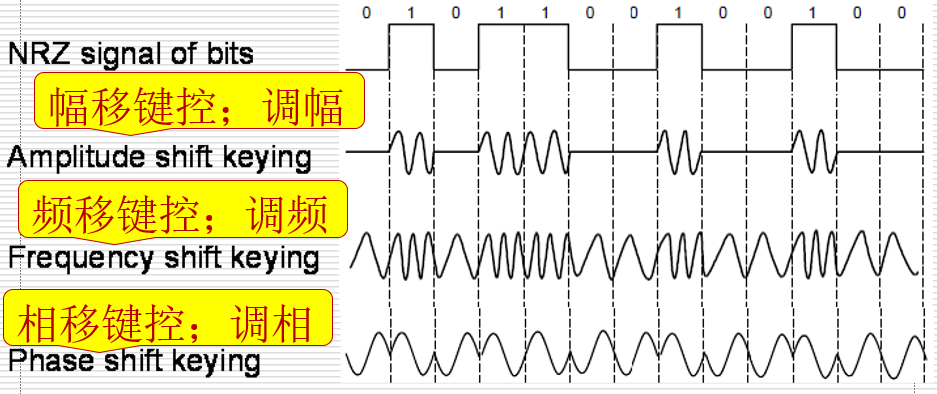
\includegraphics[scale = 0.3]{assets/jisuanjiwangluo_2eccd.png}
    \caption{通带传输}
  \end{figure}
\begin{itemize}
  \item 调幅,使用不同振幅表示信号,振幅为1表示1,没有振幅表示0
  \item 调频,使用不同频率载波信号表示振幅
  \item 调相:使用不同相位表示0和1
\end{itemize}

\begin{figure}[H]
  \centering
  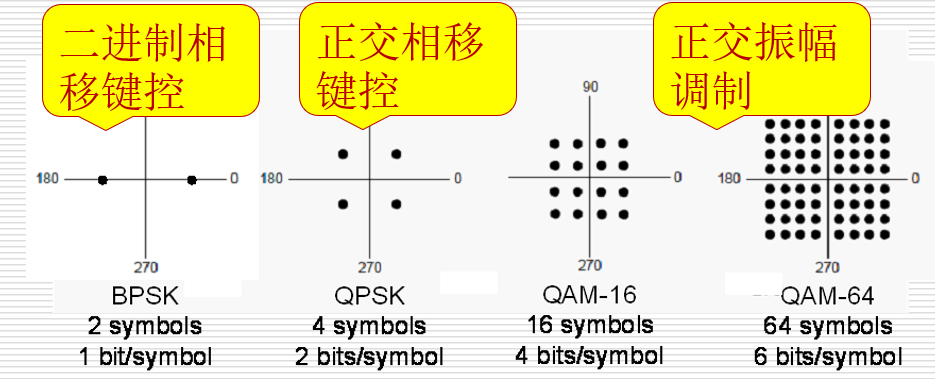
\includegraphics[scale = 0.3]{assets/jisuanjiwangluo_fe463.png}
  \caption{信号星座}
\end{figure}

  通带传输3种情况的综合应用:使用不同相位、波长表示不用的信号,这样接受一个符号,这个符号能表示的范围就变大,从而减少传输的时间。\\
  比如每次接受一个波形,能可能表示4个情况,那么这个波形就能表示两个位(00,01,10,11)的一种

  \subsubsection{复用技术}
  复用技术:多个用户使用同一个通道。\\
  前面相位、波长用来表示数字,而频率和其他冗余信息则主要用于复用技术方面。

  复用技术主要有以下几种类型:
  \begin{itemize}
    \item 频分多路复用(FDM):
    不同频率直接叠加,最终经过滤波器分开
    \item 正交FDM OFDM:
    普通的FDM每个频率段之间是不交的,而正交FDM有相交部分,但是也能区分开来
    \item 波分多路复用 WDN:和FDM一样
    \item 时分多路复用:
    时间上共享,一个接一个使用
    \item 统计时分多路复用 STDM:
    时分多路复用的话,是每个用户一次分配到使用时间,不管有没用到,而统计时分多路复用则是没有用到就不分配时间
    \item 码分多路复用 CDMA:\\
    码元:承载信息量的基本信号单位,常使用时间间隔相同的符号来表示二进制数字
    每个用户拥有一个唯一的码片,每个码片相互正交(主要用于3G网络)\\
    比如,传送4位信号,里面能包含3个用户发送的信息情况等。
    \begin{figure}[H]
      \centering
      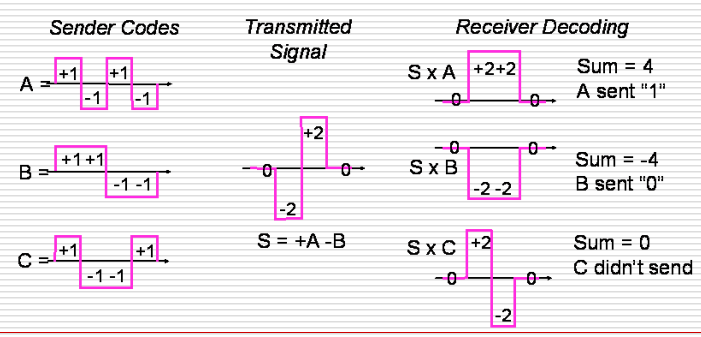
\includegraphics[scale = 0.3]{assets/jisuanjiwangluo_93b08.png}
    \end{figure}
  \end{itemize}

  \begin{figure}[H]
    \centering
    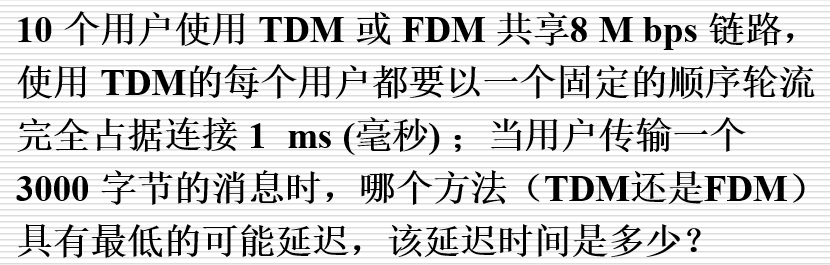
\includegraphics[scale = 0.3]{assets/jisuanjiwangluo_ee1de.png}
    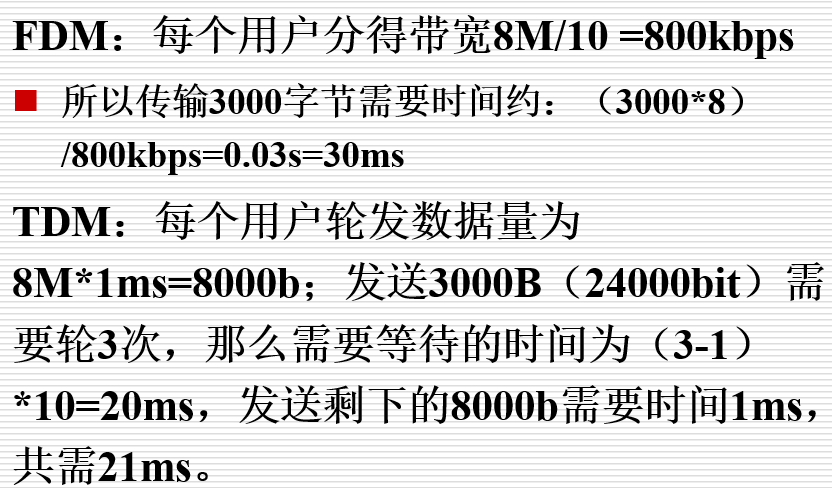
\includegraphics[scale = 0.3]{assets/jisuanjiwangluo_a7c97.png}
    \caption{也就是TDM不用考虑发送完之后那个周期的剩余时间(9ms)}
  \end{figure}

  \subsection{物理层设备与冲突域}
  \begin{itemize}
    \item 被动设备:接线板,插头,插座,电缆
    \item 主动设备:转发器(网卡的部分),中继器(再生信号:去噪和放大信号),集线器
    \item 冲突: 同时发送数据,引起冲突
  \end{itemize}

  怎么防止冲突?减小冲突域

  中继器和集线器会扩大冲突域

  \subsection{公共电话交换网络 PSTN}
  PSTN:public switched telephone network

  \textbf{主要构成及技术}:本地回路(调制技术) , 干线及复用技术 , 交换

  \begin{figure}[H]
    \centering
    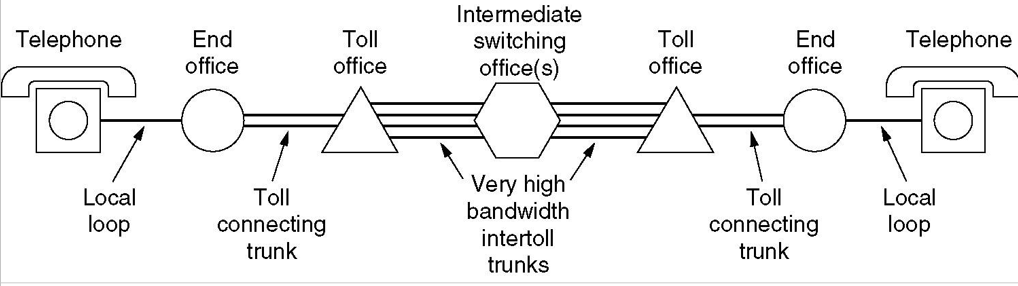
\includegraphics[scale = 0.3]{assets/jisuanjiwangluo_3aee3.png}
    \caption{一个中距离电话的典型路径}
  \end{figure}

  \begin{itemize}
    \item 本地回路:模拟线路,调制技术,用户到交换局
    \item 干线:数字光纤,连接交换局,采用复用技术
    \item 交换局:话音接驳干线的场所
  \end{itemize}

  \textbf{调制解调器:}数字信号$\to$模拟信号


  \begin{figure}[H]
    \centering
    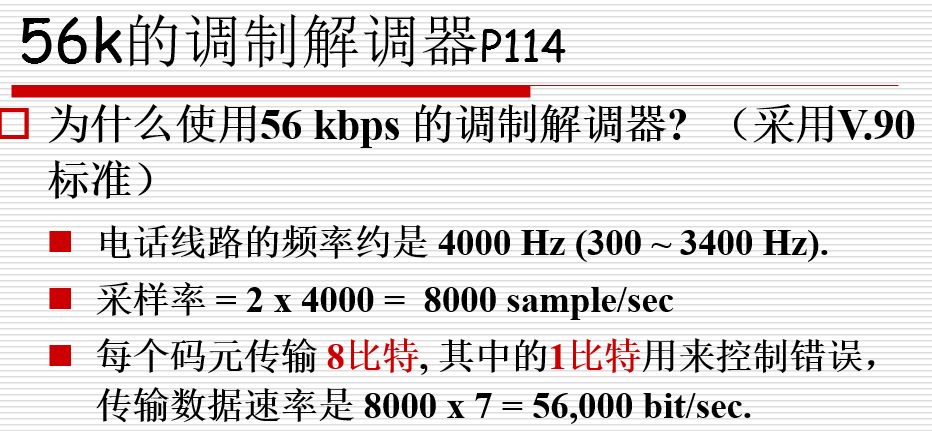
\includegraphics[scale = 0.3]{assets/jisuanjiwangluo_460b3.png}
  \end{figure}

  \textbf{xDSL}: modem带宽低,xdsl本地回路使用全部的1.1Mhz,宽带能达到8M

  \textbf{TCM}: 每次采样中,有一位用于纠错

  \begin{figure}[H]
    \centering
    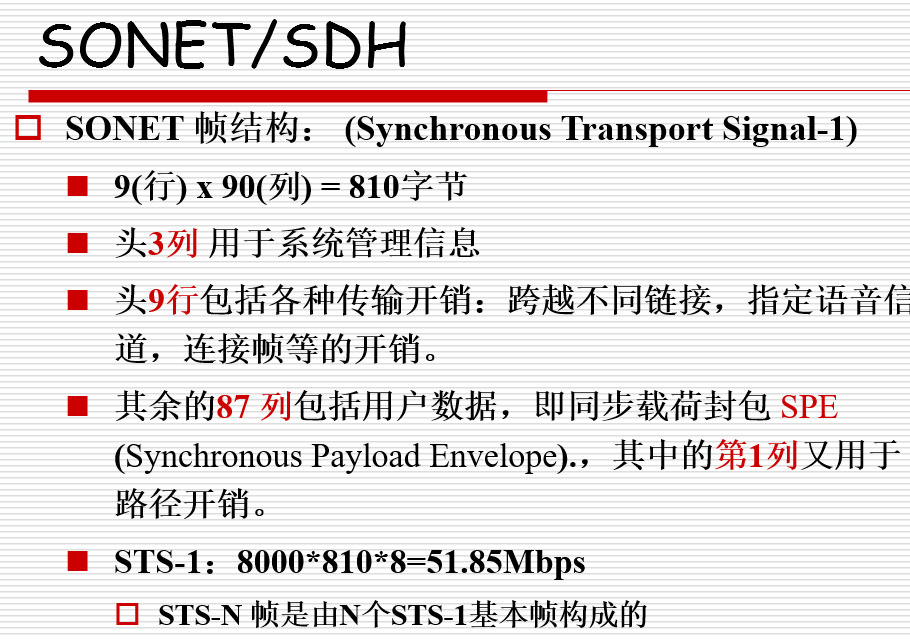
\includegraphics[scale = 0.3]{assets/jisuanjiwangluo_b4683.png}
    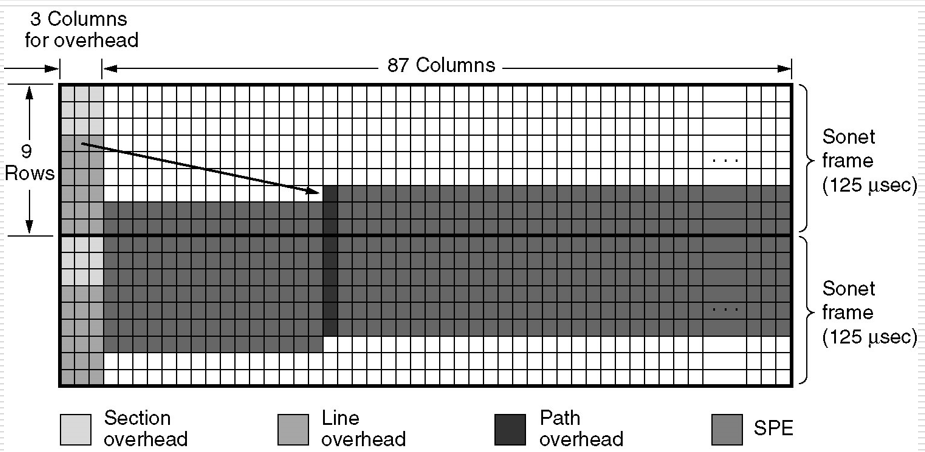
\includegraphics[scale = 0.3]{assets/jisuanjiwangluo_25858.png}
    \caption{干路复用技术 SONET}
  \end{figure}


  \begin{figure}[H]
    \centering
    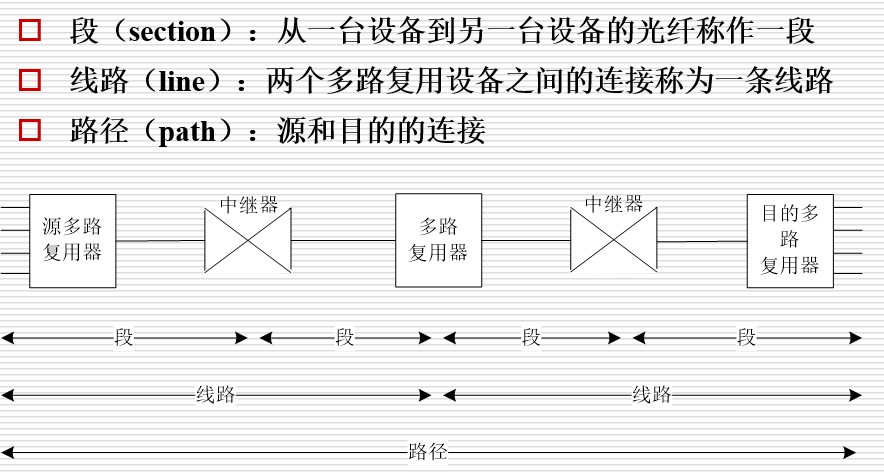
\includegraphics[scale = 0.3]{assets/jisuanjiwangluo_b52d1.png}
    \caption{段、线路、路径}
  \end{figure}

  除了北美和日本,其他国家使用E1系列线路:
  \begin{itemize}
    \item E1可以处理 \textbf{32} 条语音的复用:$32\times 8 = 256 bits/frame$
    \item 予以按采样率是每秒 \textbf{8000} 次
  \end{itemize}
  \begin{figure}[H]
    \centering
    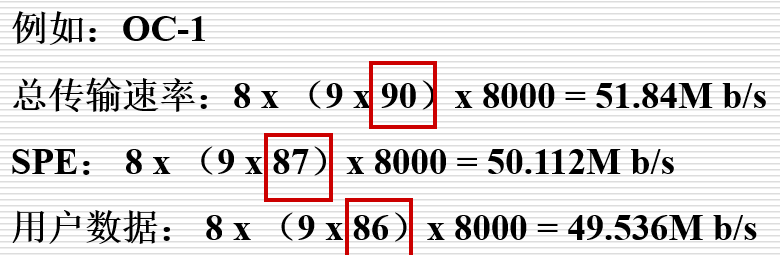
\includegraphics[scale = 0.3]{assets/jisuanjiwangluo_91e6a.png}
    \caption{8000是采样率;OC-12 指的是 Optimal Carrier , 结果是OC-1的数值$\times$12}
  \end{figure}

  \textbf{交换}:
  \begin{itemize}
    \item 电路交换:双方打通通道
    \item 报文交换: 同分组交换
    \item 分组交换:每个分组独立寻径,直接投放数据(分组交换的分组有大小限制,而报文没有)
  \end{itemize}

  \section{数据链路层}
  数据链路层的作用:
  \begin{itemize}
    \item 为网络层提供服务,良好的服务接口
    \item 保证数据传输的有效、可靠:处理传输错误(差错检测和控制);流量控制(基于速率,基于反馈)
  \end{itemize}

  \textbf{确认}:接受方收到数据帧后,必须给发送方发回一个确认

  \textbf{面向连接}:发送发和接收方在传输数据之前必须建立逻辑连接,传输结束后必须释放连接

  \textbf{服务种类:}无确认无连接服务;有确认无连接服务;有确认的面向连接服务

  无确认并非不可靠,可靠新由上层协议负责

  \subsection{成帧}
  数据链路层使用物理层提供的服务,物理层处理的是 \textbf{位流} ,数据链路层处理的是 \textbf{帧}

  将原始的位流分散到离散的帧中,叫成帧,成帧的方法有:
  \begin{itemize}
    \item 字符计数法\\
    	帧头为字节长度,一旦出错,后续完全错误,无法恢复 , 很少使用
      \begin{figure}[H]
        \centering
        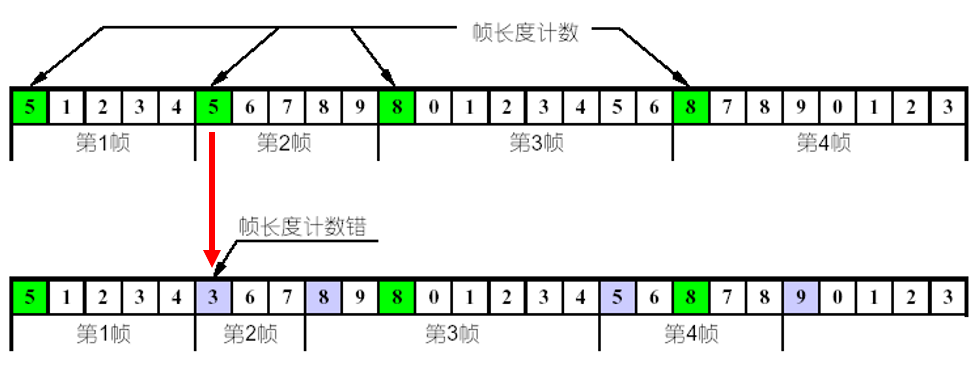
\includegraphics[scale = 0.3]{assets/jisuanjiwangluo_d37e3.png}
        \caption{字符计数法}
      \end{figure}
    \item 带字节/字符填充的标志字节法\\
    	使用特殊的字节(flag byte)作为字节作为帧的开始,需要定义转义字节来在数据中使用这个特殊的字节
      \begin{figure}[H]
        \centering
        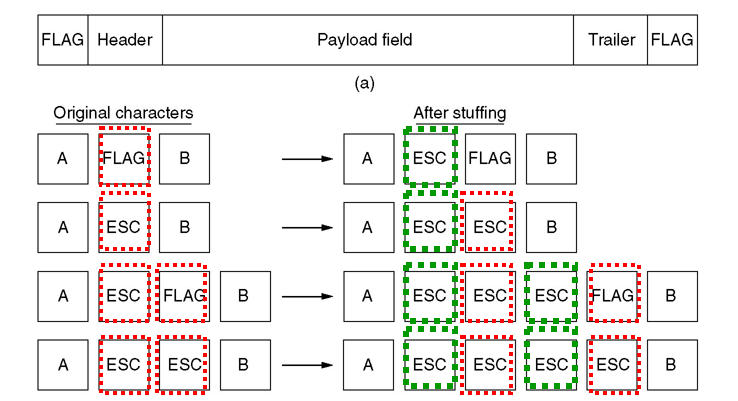
\includegraphics[scale = 0.3]{assets/jisuanjiwangluo_877b1.png}
        \caption{字节填充的标志字节法}
      \end{figure}
      缺点:依赖于8位字符
    \item  比特填充的比特标志法(零比特传输,透明传输)\\
    	以特殊的位模式作为帧的开头,比如01111110(0+6个1+0),如果要数据和帧头一样,则在第5个1后面加个0,
    	这样就能保证数据一定不会出现6个1,当出现5个1的时候,自动把后面的0去掉
    \item 物理层编码违例法\\
    	在曼彻斯特编码张,只有电压跳变是数据,那么可以使用 高高,或者低低这样的电平作为帧的边界\\
      使用跳变作为数据,使用连续高/低电平作为帧的边界
  \end{itemize}


  \subsection{差错控制}
  \textbf{差错的类型} :单个错误;突发错误

  通常利用处理单个错误的方法来应对突发错误

  \textbf{差错处理} :纠错(主要用于无线网络中),检错
  \begin{itemize}
    \item 纠错码:发现错误,从错误中回复正确的数据,主要用于无线网络
    \item 检错码:只能发现错误,不能从错误中恢复,但可采用重传
  \end{itemize}

  \subsubsection{纠错}

  \textbf{码字} :包含数据位和校验位的n位单元

  \textbf{两个码字海明距离} :两个码字不同位的数目

  \textbf{全部码字的海明距离} :最小的海明距离

  \textbf{海明距离}:如果海明距离为d,则一个码字需要发生d+1位错误才能变成另一个码字

  \begin{itemize}
    \item 海明距离为d+1的编码能检测出d位错误
    \item 海明距离为2d+1的编码,能纠正d位错误(恢复成最近的海明吗)
  \end{itemize}

  \textbf{纠一位错的海明码}

  纠一位错需要多少位冗余位?

  冗余为r位,数据为m位, 纠一位错误:数据有$2^m$种可能,每条数据都有各自的$m+r$个距离为1的错误的码,算上它自己,算上所有的数据可能,那么总共有$(m+r+1)2^{m}$ ,而总的数据有$2^{m+r}$种可能,那么要求$(m+r+1)2^{m} \leq 2^{m + r}$

  得:$m + r + 1 \leq 2^r$

  由此不等式,我们可以求出,在给定m的条件下,至少需要多少(r位)校验位

  \textbf{纠一位错的海明码}:编号位2的幂的位都是数据位,每一位表示包括自己在内的一些位集合奇偶值(编号从1开始)

  那么这些位集合怎么取?把编号按2的幂求和展开,这一编号所代表的位,就要参与这些2的幂对应的校验位的奇偶计算

  \textbf{检错:} 校验位不对的就是了,逐个检查每个校验位的奇偶性

  \textbf{纠错:}一个位出错,会影响到所有它所在的集合对应校验位,因此只要对出错的校验位的编号进行累加,得到的编号,就是出错的位的编号

  \textbf{优化} :连续k个码字按行排列成矩阵,按列发送,注意,列没有海明编码,就是按列直接发送

  当出现突发错误的时候,发送的一列都出错了,对于一行来说,只有一位发生错误,也能根据行的海明码进行纠错
  \begin{figure}[H]
    \centering
    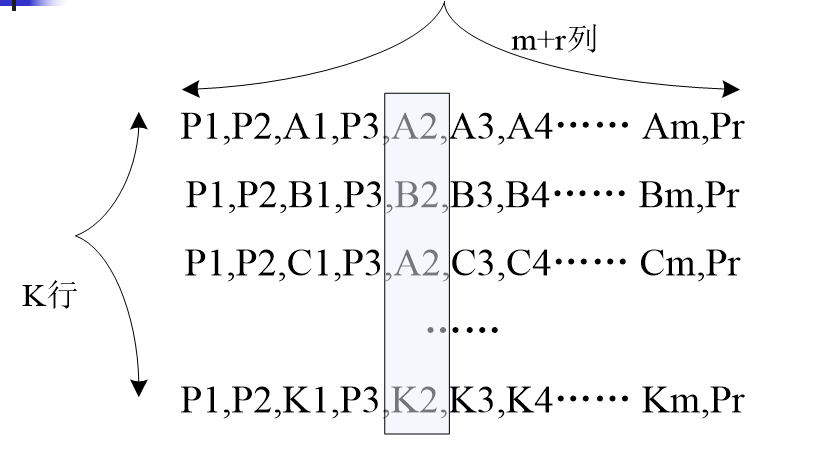
\includegraphics[scale = 0.3]{assets/jisuanjiwangluo_55419.png}
    \caption{优化}
  \end{figure}

  \begin{figure}[H]
    \centering
    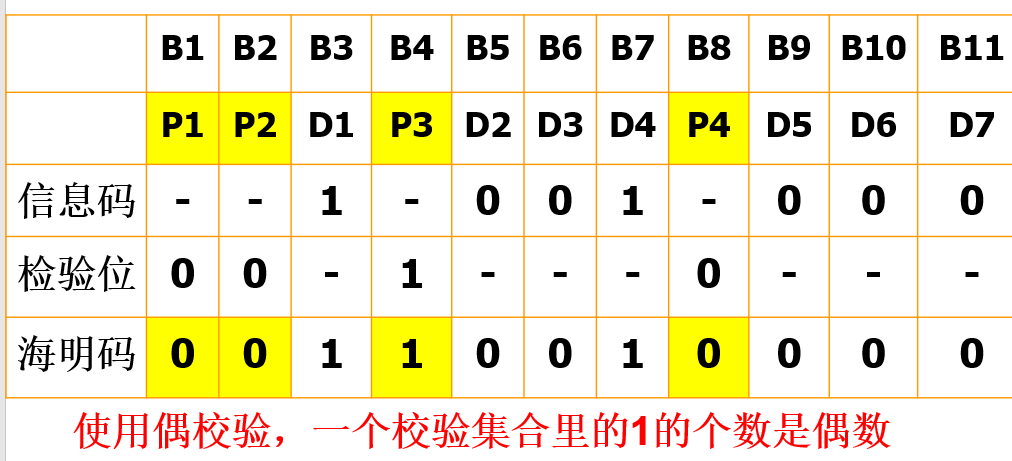
\includegraphics[scale = 0.3]{assets/jisuanjiwangluo_b5d1f.png}
    \caption{海明码例子1:采用偶校验}
  \end{figure}

  \begin{figure}[H]
    \centering
    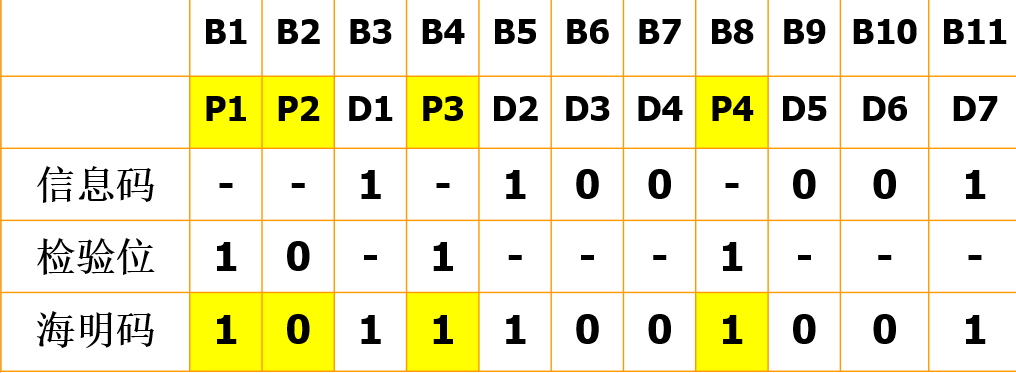
\includegraphics[scale = 0.3]{assets/jisuanjiwangluo_0f780.png}
    \caption{海明码例子2:采用偶校验}
  \end{figure}

  \begin{figure}[H]
    \centering
    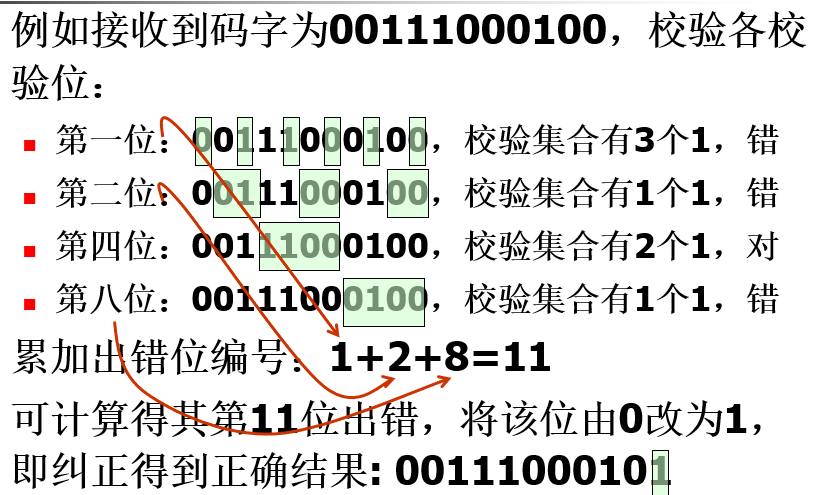
\includegraphics[scale = 0.3]{assets/jisuanjiwangluo_49c7c.png}
    \caption{海明码纠错例子}
  \end{figure}

  \begin{figure}[H]
    \centering
    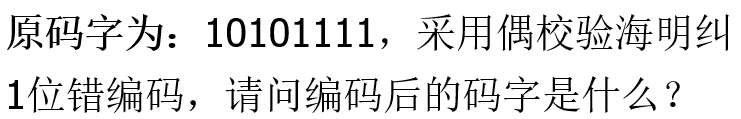
\includegraphics[scale = 0.3]{assets/jisuanjiwangluo_8ebde.png}
    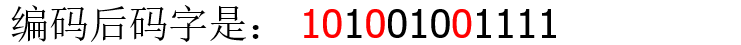
\includegraphics[scale = 0.3]{assets/jisuanjiwangluo_8afbd.png}
    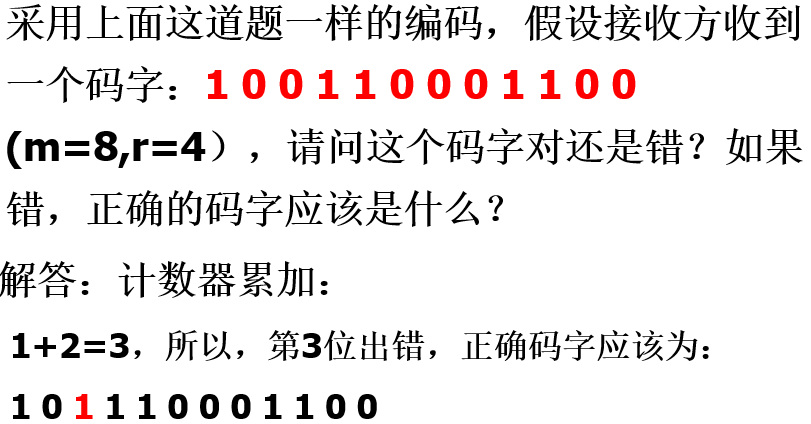
\includegraphics[scale = 0.3]{assets/jisuanjiwangluo_3de51.png}
  \end{figure}

  \subsubsection{检错}
  检错码仅包含接收方检查出是否有错误的足够信息,如果物理层的错误率(铜线或光纤)足够低,采用检错和重传机制更加有效

  \textbf{奇偶校验} :保证码字的1的个数是奇/偶数个,但只能检测出奇数个错误(海明距离为2,检1位错)

  \textbf{校验和}:校验和通常是按N位码字来模拟模2和运算,发放将运算结果附加在数据报文尾部, 作为校验位
  \begin{itemize}
    \item 比奇偶校验更好的检错性能
    \item 能检出高至N位的突发错
    \item 检错随机率 $1-2^N$
    \item 易受系统错误干扰,比如,增加的 "0"
  \end{itemize}
  \begin{figure}[H]
    \centering
    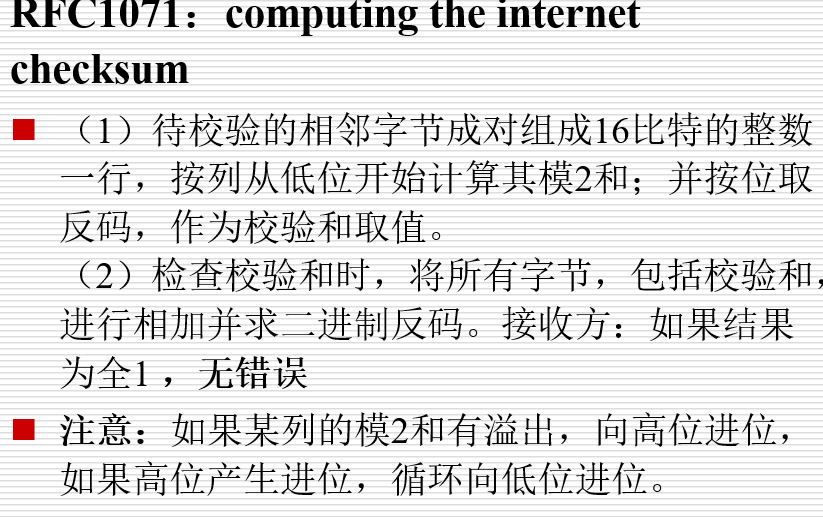
\includegraphics[scale = 0.3]{assets/jisuanjiwangluo_08665.png}
    \caption{互联网校验和计算文档}
  \end{figure}


  \textbf{CRC循环冗余检错码}:
  任何一位k位的帧,可以看成是 \textbf{k-1} 位的多项式,比如101表示x\^2 + x\^0

  设定一个生成多项式G(x),G(x)是r阶,
  假设数据为M(x) , 则发送 x\^rM(x)+ R(x) , R(x)为x\^rM(x)/G(x)的余数,从编码来看就是T(x) = 【M(x) , R(x)】
  接收方收到的时候,T(x)/ G(x),能整除,则说明没有出错

  注:上面提到的加减运算都是 模二加减(异或),不进位也不借位

  \begin{figure}[H]
    \centering
    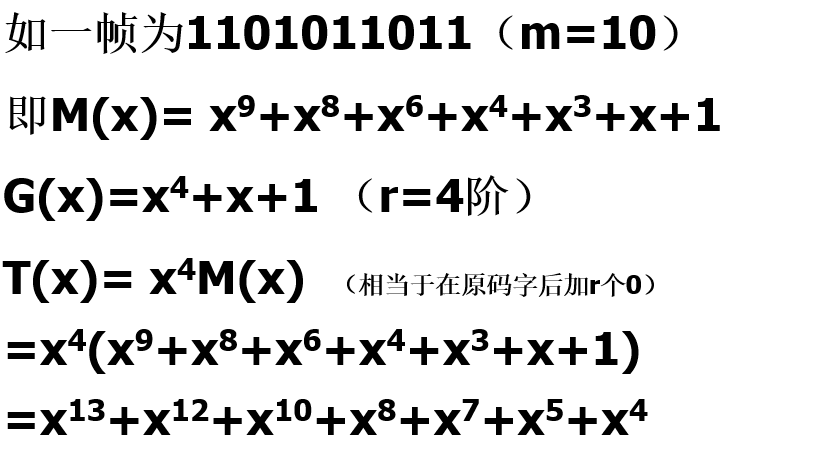
\includegraphics[scale = 0.3]{assets/jisuanjiwangluo_64318.png}
    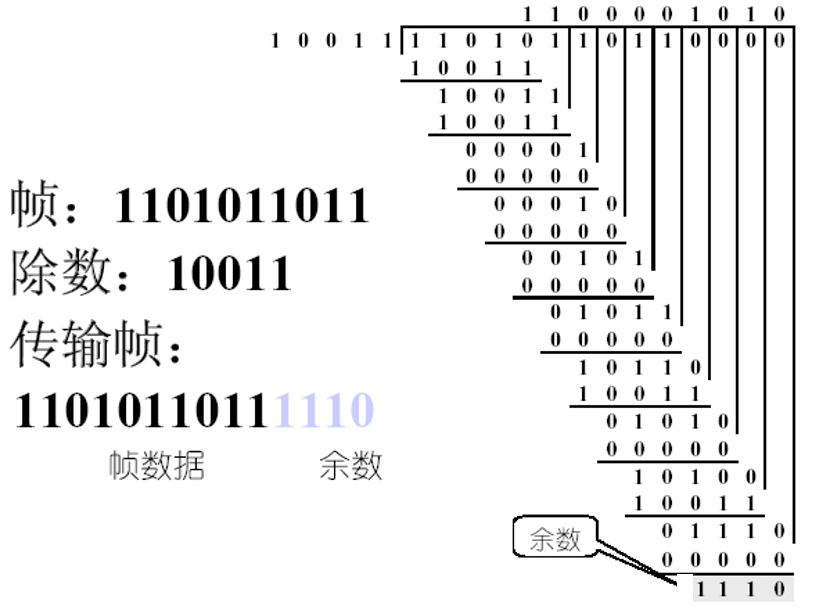
\includegraphics[scale = 0.3]{assets/jisuanjiwangluo_05982.png}
    \caption{CRC码计算距离}
  \end{figure}

  例子:多项式1101 , 待发送1111和1100,编码之后是多少?
  1111111和1100101

  \subsection{6个基本链路协议}
  几个假设:
  \begin{itemize}
    \item 物理层、数据链路层和网络层各自是独立的处理进程
    \item 机器A希望向机器B发送的是一个可靠的、面向连接的长数据流
    \item 假设机器不会崩溃
    \item 从网络层拿到的数据是纯数据
  \end{itemize}
  \subsubsection{无限制的单工协议}
  协议1的假设:
  \begin{itemize}
    \item 1. 数据单向传输
    \item 2. 收发双方的网络层都处于就绪状态,(随时待命)
    \item 3. 粗粝时间忽略不计(瞬间完成)
    \item 4. 可用的缓存空间无限大(无限空间)
    \item 5. 假设DLL之间的信道永远不会损坏或者丢失数据帧(完美通道)
  \end{itemize}

  协议1:发送方不断发,收方不断收
  \subsubsection{单工停-等协议}
  协议2:解决如何避免收方被涌入的数据淹没,即取消"接收方允许无限量接受"的假设

  考虑接收方的处理能力有限(缓存有限)

  实际上是半双工协议,而不是单工协议

  发送方发送之后等待接收方回复的哑帧才继续发下一个数据帧

  \subsubsection{有噪声信道的单工协议}
  协议3:
  信道不是完美的,可能丢失帧也可能接收到错误帧
  \begin{itemize}
    \item 1. 对正确帧的确认(确认帧丢失,发送方超时重发,接收方拒收(根据编号判断),但是重发确认帧)
    \item 2. 超时重传(可以防止死锁的产生,就是A发送B,等待B确认,结果帧丢失,A依旧等待B发送,变成双方互相等待)
    \item 3. 对帧进行编号(当确认帧丢失以后,发送方重发,而接收方接收之后还需要判断是重发的还是新的帧,因此需要编号)
  \end{itemize}

  小结:超时可能是数据帧丢失也可能是确认帧丢失

\subsubsection{滑动窗口协议}
如果发送端可连续发送一批数据帧,必须考虑接收端是否来得及接纳和处理这么多帧, 这里提出了网络流量控制问题

\textbf{流量控制机制:} 在接收方缓冲区达到一定一定量时,应及时通知发送方,暂停发送,等候通知

\textbf{滑窗协议} (协议4~6)

原理:当接收方收到帧之后,先核对是否是预期帧号,是则移动接收窗口,并返回确认帧;发送方收到应答帧,核对响应帧号,是则移动发送窗口
\begin{itemize}
  \item 协议4:n = 1 引出滑动窗口的技术
  \item 协议5-6:滑动窗口对出错帧的两种应对措施
\end{itemize}

\begin{itemize}
  \item 全双工:双方可以互相发送提高效率
  \item 捎带确认:确认帧放在接收方下次发送的帧,如果没有才发送哑帧
  \item 批发数据:多个数据帧同时发送(滑动窗口)
\end{itemize}

\subsubsection{协议4}
双方互相发送 + 捎带确认 + 窗口大小为1,n = 1

发送窗口:对应已经发送但还未被确认的帧的序号,当接收到确认之后窗口滑动,发送下一帧

接收窗口:对应期望接收的帧的序号,收到期望的帧,滑动窗口


异常:
\begin{itemize}
  \item 1. 定时器设短了,能正常工作,但是会发送大量的重复帧,
  \item 2. 同时发送,能正常但重复(数据接收没问题,但是确认帧号不对,因此接收到的会重发一次数据)
\end{itemize}

\textbf{信道利用率计算} :
信道传输速率b bps,帧大小k bit,来回时间R s

则信道利用率:$\frac{k}{k + Rb}$(实际发送数据 / 最大可发送数据)

发送过程:发送k,然后等待Rs确认

\begin{figure}[H]
  \centering
  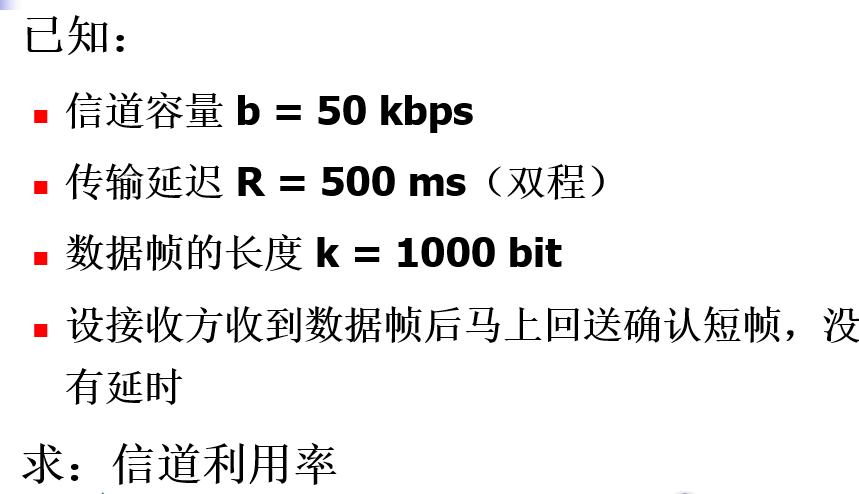
\includegraphics[scale = 0.3]{assets/jisuanjiwangluo_6ec33.png}
  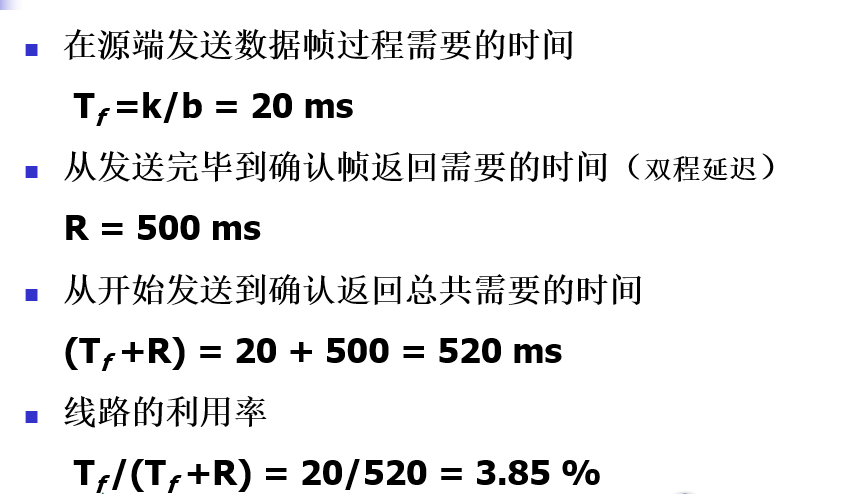
\includegraphics[scale = 0.3]{assets/jisuanjiwangluo_a9eea.png}
  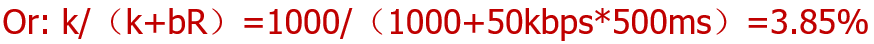
\includegraphics[scale = 0.3]{assets/jisuanjiwangluo_4b94f.png}
\end{figure}


\textbf{提高信道利用率}:管道化技术

滑动窗口长度增加到W,即一次发送W个数据帧

信道利用率为:$\frac{W*k}{(k + Rb)}$(是利用发送一帧的空闲部分发送剩余W-1帧,因此分母是k)

令上式=100\% ,可以得到信道利用率为100\%下的W

\textbf{怎么寻找一合适的W的值?}
宽带延迟积:bd,信道上的容量:一帧从发送方传输到接收期间可容纳的帧数量 bd = bandwidth * delay

窗口值:w = 2*bd + 1

2表示往返两个方向的时间,+1表示呆在网卡上的还没发送出去的一帧

\begin{figure}[H]
  \centering
  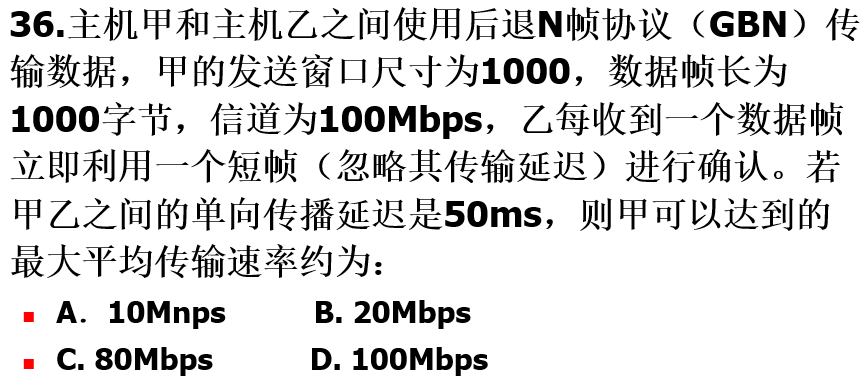
\includegraphics[scale = 0.3]{assets/jisuanjiwangluo_13ba7.png}
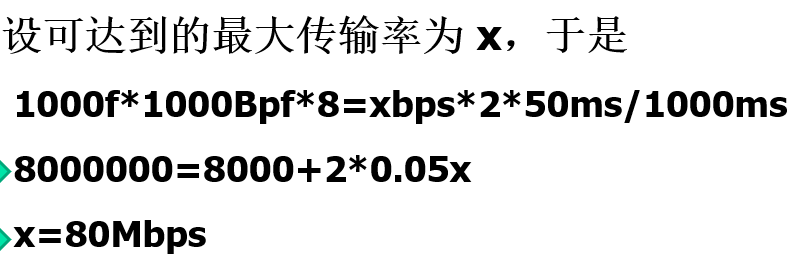
\includegraphics[scale = 0.3]{assets/jisuanjiwangluo_43d86.png}
  \caption{2014考研题:最大发送1000个窗口 , 时间为50*2 , 求速度}
\end{figure}

那么,如果帧 \textbf{出错了} ,怎么处理?连续发送w个数据帧, 其中一帧出错, 但其后帧被成功发送

\textbf{接收方策略}:
\begin{itemize}
  \item 丢弃错误的帧以及后续非期望接收的帧(协议5)
  \item 丢弃错帧,缓存后续正确接收帧(协议6)
\end{itemize}

\textbf{对应发送方的重传策略:}
\begin{itemize}
  \item 缓存在发送窗口中的出错数据以及其后续的帧全部重发(协议5)
  \item 只重发错帧(协议6)
\end{itemize}

\subsubsection{协议5:回退n帧}
\textbf{接收方策略}:丢弃错误的帧以及后续非期望接收的帧(协议5)

\textbf{对应发送方的重传策略:}缓存在发送窗口中的出错数据以及其后续的帧全部重发(协议5)

\begin{itemize}
  \item 接收窗口大小为1,再大也没用
  \item 对错误帧不确认
  \item 定义序列号seq的取值范围和滑动窗口长度W
  \item 发送方超时重传,从未被确认帧开始
\end{itemize}

\begin{figure}[H]
  \centering
  \includegraphics[scale = 0.3]{assets/jisuanjiwangluo_f16d6.png}
\end{figure}

接收窗口大小 : $W = MAX\_SEQ$

异常:$W > MAX\_SEQ$时 ,若 $MAX\_SEQ = 7$, 对第0帧的确认 , 可能会被误判为对第8帧(编号也为0)的确认

\begin{itemize}
  \item 发送方需要较大的缓冲区 , 以便重传
  \item 重传帧比较多 ,适合信号出错率较少的情况
\end{itemize}

\subsubsection{协议6:选择重传协议}
\textbf{接收方策略}:丢弃错帧,缓存后续正确接收帧(协议6)

\textbf{对应发送方的重传策略:}只重发错帧(协议6)

\begin{itemize}
  \item 接收窗口只存储差错帧后继的所有正确帧
  \item 发送发只重传差错帧
  \item 接收方接收重传帧 , 按正确顺序将分组提交网络
  \item 每接收到一个非期望帧 , 发送一NAK , 加速出错帧的重传 , 使发送方不再等待超时重传
\end{itemize}

\begin{figure}[H]
  \centering
  \includegraphics[scale = 0.3]{assets/jisuanjiwangluo_a74df.png}
  \caption{选择重传协议的工作原理分析}
\end{figure}

接收窗口大小:  $W = (MAX\_SEQ + 1) / 2$ , 序列号从$0\to MAX\_SEQ$ , 发送窗口和接收窗口同大

异常 :$W >  (MAX\_SEQ + 1) / 2$时 , 重传的出发有两种可能,一个是接收到NAK , 一个超时 , 触发超时可能是因为最后一帧的确认帧的丢失 , 而此时接收方已经把帧提交给上一层 ,
此时等待接受新的帧, 而对于发送方来说,它要重发旧帧, 由于旧帧和待接受的新帧编号一致 , 就导致了错误。即错误的原因是由于新的窗口的编号和旧的窗口的编号有重叠, 主要保证编号不重叠就不会发生这个问题 ,因此滑动窗口要取$W >  (MAX\_SEQ + 1) / 2$

\begin{figure}[H]
  \centering
  \includegraphics[scale = 0.3]{assets/jisuanjiwangluo_e889b.png}
\end{figure}

\begin{itemize}
  \item 接收方需要较大的缓冲区 ,以便按正确顺序将分组提交给网络层
  \item 重传帧数少 ,适于信道质量不好的情况
\end{itemize}

采用累计确认,当帧好n的确认到底时,其之前的帧也成功接收(这个是对发送方而言,如果接收到n的确认,n-1的确认丢失了也没关系)
(同时会发接收到的最后一帧的确认,这句感觉是废话啊,不是收到就确认了吗?其实不是,丢弃一个就确认一次,因此不是接收完就确认,
而是接收到下一帧错误的时候才确认,那么正常情况下hi怎么确认的呀?
正常是接收到最大的序列号就确认)

\begin{figure}[H]
  \centering
  \includegraphics[scale = 0.3]{assets/jisuanjiwangluo_3b720.png}
  \caption{3个协议窗口大小小结}
\end{figure}

\begin{figure}[H]
  \centering
  \includegraphics[scale = 0.3]{assets/jisuanjiwangluo_1d115.png}
  \includegraphics[scale = 0.15]{assets/jisuanjiwangluo_af4a9.png}
\end{figure}

\begin{figure}[H]
  \centering
  \includegraphics[scale = 0.3]{assets/jisuanjiwangluo_aa2b2.png}
\end{figure}

\begin{figure}[H]
  \centering
  \includegraphics[scale = 0.3]{assets/jisuanjiwangluo_4517d.png}
\end{figure}

\begin{figure}[H]
  \centering
  \includegraphics[scale = 0.3]{assets/jisuanjiwangluo_dff1f.png}
\end{figure}

\subsection{点到点协议 PPP协议}
前6个都是模拟协议 , PPP协议,点到点协议 Point to Point Proocal

PPP是一种在链路上传输分组的常用方法:
\begin{itemize}
  \item 采用字节填充的帧界法(0x7E)
  \item 无序号帧(无确认无连接)用于承载IP分组
  \item 采用校验和检错\\
  使用Internet校验和(4位字),按照4位1行进行排列,按列相加,低位开始相加(模2加);产生进位,向高位进,最高位产生进位,向最低位循环进位
\end{itemize}

\begin{figure}[H]
  \centering
  \includegraphics[scale = 0.3]{assets/jisuanjiwangluo_4ef98.png}
  \caption{PPP帧格式}
\end{figure}

传输之前需要认证,两种认证方法:
\begin{itemize}
  \item PAP:2次握手,传送账号密码,接收方检查后接收或拒绝\\
  不足:明文传送, 可以不断尝试密码,造成DOS攻击,拒绝服务攻击
  \item CHAP:3次握手,由中心节点发送一个随机数,再等待对方回复,根据对方的回复决定是否接收或拒绝对方
\end{itemize}

发送:0x7E,先使用0x7D填充,再发送 0x7E XOR 0x20 即0x5E

接收:扫到0x7D就丢弃,后面的数字xor 0x20(这也是为什么0x7D是 0x 7d 0x 5d)

地址固定为11111,因为点到点传输,对方的地址是非常明确的,因此不用设置地址。控制0011表示无确认无传输

protocal:BIAOSHI表示上层协议

\section{介质访问子层}
数据链路层分为两个子层:LLC Logical Link Control,MAC Madia Access Control
\begin{figure}[H]
  \centering
  \includegraphics[scale = 0.3]{assets/jisuanjiwangluo_d896b.png}
  \caption{介质访问控制子层的位置}
\end{figure}



广播需要解决的问题: 可能存在两个或更多的站点同时请求占用信道

解决办法:介质的多路访问控制 , 在多路访问信道上确定下一个使用者

\textbf{怎么分配信道?(介质访问控制)}
\begin{itemize}
  \item 静态分配 : 只有一个站 / 用户 使用信道 , 不用就浪费了 ; 频分多路复用 FDM ; 时分多路复用 TDM;\\
  问题:资源分配不合理 , 不满足用户对资源占用的不同需求 ; 有资源浪费 , 效率低 ; 延迟时间增大N倍

  适用情况 : 适于用户数量少且用户数量稳定的情况 ; 适用通信量大且流量稳定的情况 ; 不适用于突发性业务的情况
  \item 动态分配 : 信道是开放的 , 没有预分配的\\
  基本思想 : 通过 多路访问协议 动态分配信道资源 , 提高 信道利用率 \\
  5个关键假设 : \textbf{流量独立} 、 \textbf{单信道} 、 \textbf{冲突可观察} 、 \textbf{载波侦听与否} 、 \textbf{帧的发送方式}

  多路访问协议:
  \begin{itemize}
    \item 随机访问协议 : 站点争用信道, 可能出现站点之间的冲突 ; \\
    典型协议 : \textbf{ALOHA协议} 、 \textbf{CSMA协议} 、 \textbf{CSMA/CD协议}
    \item 受控访问协议 : 站点被分配占用信道 , 无冲突
  \end{itemize}

\end{itemize}

\subsection{ALOHA协议}

ALOHA协议:想什么时候发送数据帧就什么时候发送

\subsubsection{纯ALOHA协议}
纯ALOHA协议:想发就发,当检测到冲突(发送失败),就延迟重发

\textbf{帧时} : 发送一个标准长的帧所需时间

\textbf{统计规律:}每个时间帧发送k个数据的帧数满足泊松分布
$P_r[k] = \frac{G^kE^{-G}}{k!}$
其中,G表示,帧时T内,信道内的帧数(包括重发的)

\textbf{吞吐率S:}在发送时间T内成功发送的平均帧数($0 < S < 1$)

\textbf{信道利用率:}T为单位时间的时候的吞吐率

\textbf{运载负载}:G,发送时间T内,总共发送所有的帧数平均值(包括原发和重发)

根据定义有:$S = GP_0$,其中$P_0$表示一帧发送成功的概率。那么问题是,$P_0$怎么求?

对于ALOHA协议,当一个发送端想要发送数据的时候,它想要发送成功,就要求发送的时间段内没有其他数据帧发送。
而发送端所占的时间,至少会有两个帧时是处于危险期(可能冲突),因此需要两个帧时都没有数据帧,根据前面的分布规律\\
$P_0 = (Pr[0])^2 = e^{-2G}$

\textbf{求吞吐率S的极大值} : $S' = e^{-2G}-2Ge^{-2G} = 0$得$G = 0.5$时 , $S = 0.184$

即 纯ALOHA协议的信道利用率最高为$18.4\%$

\subsubsection{分槽ALOHA协议}
分槽ALOHA协议:只有时间片开头才发送帧,冲突发生会浪费一个时间槽(把冲突时间降低为1个t,而不是纯ALOHA的2个t)
\begin{itemize}
  \item 时间分槽,只有在时间槽开始的时候才能发送数据帧
  \item 一个时间槽只有一个帧,那么这一帧一定能成功发送
  \item 多个帧发送,那么均发送失败,这个时间槽作废
  \item 时间槽一般取帧时
\end{itemize}

而对于分槽的ALOHA协议,只要没有其他人抢占帧时,那么就一定能发送成功,因而只需要考虑一个帧时内没有数据帧即可,因此\\
$P_0 = Pr[0] = e^{-G}$

\begin{figure}[H]
  \centering
  \includegraphics[scale = 0.3]{assets/jisuanjiwangluo_ab468.png}
  \caption{ALOHA吞吐率和G之间的关系}
\end{figure}

$ALOHA$协议的应用:电缆传送数据 , 基站之间发送数据 , 多个RFID与RFID读写器

\subsection{CSMA协议 载波侦听多路访问协议}
\subsubsection{CSMA协议}

CSMA协议 载波侦听多路访问协议:先听后写(改进的ALOHA协议)\\
当一个站有数据要发送的时候,首先看线路上是否有其他线路发送数据
\begin{itemize}
  \item 非坚持\\
  先监听,介质空闲,开始发送,如果忙就等待随机时间,然后重复
  (随机浪费资源)
  \item 坚持\\
  先监听,介质空闲就发送,如果忙就持续监听,一旦有空就发送
  (多人等待就会冲突)
  \item p-坚持\\
  前两种的这种,当信道空闲的时候,有p的概率发送,有1-p的概率继续等待随机时间(为了避免抢占信道时候的冲突)
\end{itemize}

这种协议,在信道忙的时候不会冲突,而当信道闲的时候,还是可能发生冲突
\begin{itemize}
  \item 第一种情况是,多个帧等待发送
  \item 第二种情况是,由于延迟问题,一个发送端抢占信道之后,另一端未能检测到继续发送而导致冲突
\end{itemize}


\subsubsection{CSMA/CD}

冲突窗口:至多需要发送来回的时间就能检测到冲突,发生冲突时间的上限 , 数值上等于最远两站传播时间的两倍

CSMA/CD(以太网使用):先听(是否空闲)后发,边听(是否冲突)边发,一旦冲突,等待随机时间,并且同时发送强化冲突信号通知其他工作站也等待随机时间

这样从结果上来看,CSMA/CD从时间上划分出了竞争期和非竞争期,竞争期(最大冲突检测时间)大家随便发直到检测冲突,然后检测到不冲突的时候,就继续发送(非竞争期)
(因为是边听边发送,所以只要渡过了竞争期,其他线路都能确定监听到发送的信号,所以后面就能安稳发送完所有数据帧)

收发冲突的标记:发送和接受到的信号不一致

要求:
\begin{itemize}
  \item 时隙宽度 = 最大冲突检测时间 : 保证一个时隙能检测最远冲突
  \item 发送帧的有效时间 $\geq$ 最大冲突检测时间 : 防止发送冲突时已经完成短帧发送而造成异常情况
\end{itemize}

\subsection{其他多路访问协议}
\subsection{位图协议}
位图协议 : 也叫预留协议 , 如有N个站点共享信道,编号为0 ~N-1,其竞争周期将分为N个时隙,每个站点占有一个时隙,如某站准备发送,则可在属于它的时隙内填入1,一个竞争周期后,则将按顺序发送,不会产生冲突
\begin{figure}[H]
  \centering
  \includegraphics[scale = 0.3]{assets/jisuanjiwangluo_27209.png}
  \caption{位图协议图示}
\end{figure}

\begin{itemize}
  \item 假设系统有N个用户 ,需要N个时隙
  \item 在低负荷条件下,如每帧的数量为d bit
\end{itemize}

\section{IEEE800系列标准与以太网}
以太网的两种类型:
\begin{itemize}
  \item 经典以太网\\
  总线拓扑, 使用集线器扩充网络\\
  使用集线器的星型拓扑结构在逻辑上相当于总线
  \item 交换式以太网\\
  星型拓扑,以交换机为中心
\end{itemize}

\begin{figure}[H]
  \centering
  \includegraphics[scale = 0.5]{assets/jisuanjiwangluo_b6529.png}
  \caption{经典以太网}
\end{figure}

\begin{figure}[H]
  \centering
  \includegraphics[scale = 0.5]{assets/jisuanjiwangluo_c2575.png}
  \caption{交换式以太网}
\end{figure}

\begin{figure}[H]
  \centering
  \includegraphics[scale = 0.5]{assets/jisuanjiwangluo_99ba0.png}
  \caption{集线器与交换机的区别}
\end{figure}

\spaceline
\textbf{以太网的命名规则:}
\begin{figure}[H]
  \centering
  \includegraphics[scale = 0.5]{assets/jisuanjiwangluo_7de21.png}
  \caption{以太网的命名规则,分段长度中,2表示200米的意思,基本单位是100米}
\end{figure}

\spaceline
\textbf{以太网的编码方式:}采用曼彻斯特编码
对于802.5采用差分曼彻斯特协议

\spaceline
\textbf{IEEE802.3与以太网帧组成的区别:}
\begin{figure}[H]
  \centering
  \includegraphics[scale = 0.3]{assets/jisuanjiwangluo_f7e24.png}
  \caption{IEEE802.3与以太网帧组成的区别}
\end{figure}

\spaceline
\textbf{802.3的帧组成:}
\begin{figure}[H]
  \centering
  \includegraphics[scale = 0.4]{assets/jisuanjiwangluo_e1f57.png}
  \caption{802.3的帧组成}
\end{figure}

\textbf{最短帧长:}64B
\begin{itemize}
  \item 帧头\\
  6B目的地址,6B源地址,2B长度
  \item 数据位\\
  最少46B
  \item 校验位\\
  4B
\end{itemize}
{\color{blue}貌似没有计算先导字段}

\spaceline
\textbf{MAC地址:}物理地址,xx:xx:xx:xx:xx:xx
\begin{figure}[H]
  \centering
  \includegraphics[scale = 0.3]{assets/jisuanjiwangluo_1fa17.png}
  \caption{MAC地址组成:前24位表示公司}
\end{figure}

\spaceline
\textbf{长度字段:}帧最短长度为64B,最大为1518B

{\color{red}为什么是64B?为什么是1518B?为什么要有最短长度?P227,第一问在后面有解答}

\spaceline
\textbf{数据字段:}最少为64B,不够则填充

\spaceline
\textbf{帧校验字段:}采用32b,CRC校验

\textbf{怎么区分到底代表类型型还是长度呢}
检查这个字段的数值:如果小于等于 1536(0x600),则是长度(802.3)字段,如果大于 1536,则表示类型(以太帧)

\textbf{为什么要大于64B?}
\begin{figure}[H]
  \centering
  \includegraphics[scale = 0.3]{assets/jisuanjiwangluo_02c3a.png}
  \caption{为什么要大于64B?}
\end{figure}

{\color{red}为什么要51.2微秒的时隙?}

\spaceline
\textbf{二进制指数后退法:}有冲突检测的载波侦听策略当冲突的时候会随机等待一段时间,那么这个时间的范围什么确定?\\
\begin{figure}[H]
  \centering
  \includegraphics[scale = 0.3]{assets/jisuanjiwangluo_d029d.png}
  \caption{第i次冲突等待时间}
\end{figure}

进一步优化:一般确认接收之后,则下一个时隙留给接收方返回确认消息,而不是进入新的一轮竞争

\subsection{快速以太网(100M)}
以太网提高负载的方法:
\begin{itemize}
  \item 提速到100M
  \item 全双工
  \item 使用交换机代替集线器
\end{itemize}

100M以太网:保留原来的帧格式、接口和偶成UI则,只是将比特时间从100ns降低到10ns(物理上表现为电缆长度为原来的$\frac{1}{10}$)

\begin{figure}[H]
  \centering
  \includegraphics[scale = 0.3]{assets/jisuanjiwangluo_7150c.png}
  \caption{100BaseT4}
\end{figure}


\begin{figure}[H]
  \centering
  \includegraphics[scale = 0.3]{assets/jisuanjiwangluo_7fbf4.png}
  \caption{100BaseTX}
\end{figure}


\section{交换机}
\textbf{网桥与交换机的关系:}就像中继器与集线器的关系

\subsection{千兆以太网(1000M)}
出现的问题:1000M以太网速度太快导致传输时间太短,进而传输的距离也短
\begin{figure}[H]
  \centering
  \includegraphics[scale = 0.5]{assets/jisuanjiwangluo_72a2b.png}
  \caption{千兆以太网解决办法}
\end{figure}

注:计算机网络中一般取$1M = 10^6 , 1K = 10^3$,存储单位采取2的指数


以太网:
\begin{figure}[H]
  \centering
  \includegraphics{assets/jisuanjiwangluo_4a63a.png}
  \caption{以太网的位置}
\end{figure}

\begin{itemize}
  \item 经典以太网(3-10M)
  \item 交换式以太网(10M,100M,1G)
\end{itemize}

以太网的命名规则:
\begin{figure}[H]
  \centering
  \includegraphics{assets/jisuanjiwangluo_d438c.png}
  \caption{以太网的命名规则}
\end{figure}

以太网采用曼彻斯特编码

怎么确定CSMA/CD的等待时间?使用二进制指数后退算法

二进制指数后退算阿飞:检测到冲突后,等待的时间以2的指数增长,等待时间设置一个上界(第10~16次),对于以太网,一个时隙是(51.2 us),16次冲突后放弃发送
\begin{figure}[H]
  \centering
  \includegraphics{assets/jisuanjiwangluo_408c6.png}
  \caption{以太网的冲突等待时间}
\end{figure}

100M以太网:保留原来10M的帧格式,只是传输距离改为原来的1/10(原来为2500m),并且采用4B/5B编码

以太网的帧格式:
\begin{figure}[H]
  \centering
  \includegraphics{assets/jisuanjiwangluo_ce52c.png}
  \caption{以太网的冲突等待时间}
\end{figure}
\begin{figure}[H]
  \centering
  \includegraphics{assets/jisuanjiwangluo_2069e.png}
  \caption{以太网的冲突等待时间}
\end{figure}

前导码:定为一个新的帧其实

目的地址/源地址:48位,MAC地址,全球唯一

长度字段:长度范围:64字节~1518字节,不包括前导码

数据字段:长度最小为46个字节,少于46个就填充

校验字段:32位的CRC校验,校验范围:目的/源地址,长度,LLC数据等字段

怎么区分是类别还是长度呢?
数值小于1536(0x600)的就是长度(802.3)字段,否则表示类型(以太帧)

最少64字节怎么计算出来的?
\begin{figure}[H]
  \centering
  \includegraphics{assets/jisuanjiwangluo_149b5.png}
  \caption{以太网的最小长度计算}
\end{figure}

二层交换:不同协议需要进行重新包装

网桥如何维护内部转发表?
\begin{itemize}
  \item 泛洪算法\\
  对于未知的(表中无记录),转发到其他所有端口
  \item 反向学习\\
  记录帧来源的MAC地址加入到转发表中
\end{itemize}

但是网络的拓扑结构是变化的,网桥怎没适应这些变化?
定期删除超时的表项,每次来一帧,就更新表项的时间戳为当前时间。

怎么利用转发表?
源LAN和目的LAN相同,则丢弃,否则查表,有的转发,无则广播


为保证安全,会使用冗余的拓扑结构(多条线),但是冗余的拓扑结构可能带来以下问题
\begin{itemize}
  \item 广播风暴\\
  广播的时候,如果拓扑结构有回路,则广播信息会不断在回路循环
  \begin{figure}[H]
    \centering
    \includegraphics{assets/jisuanjiwangluo_4887c.png}
    \caption{广播风暴}
  \end{figure}
  \item 多帧传送\\
  一个接收点,会接受到多个相同的帧
  \begin{figure}[H]
    \centering
    \includegraphics{assets/jisuanjiwangluo_ac9fa.png}
    \caption{多帧传送}
  \end{figure}

  \item MAC地址库不稳定\\
  因为多条路径,源帧的MAC地址库不稳定,导致转发的行为不稳定
  \begin{figure}[H]
    \centering
    \includegraphics{assets/jisuanjiwangluo_a3aec.png}
    \caption{MAC地址不稳定}
  \end{figure}
\end{itemize}

解决办法:生成树协议,使用生成树打断环路,生成逻辑上无回路的树,但是不能保证路径最优
\begin{itemize}
  \item 每个网络选择一个根网桥
  \item 每个网桥有一个根端口
  \item 每个网段一个指定端口
  \item 非指定端口不被使用\\
  逻辑上禁用端口,虽然这个端口虽然不使用,但是还会参与侦测,当出现短路,马上启用新的端口
\end{itemize}

虚拟局域网:逻辑上的设备等同于物理上的LAN
\begin{figure}[H]
  \centering
  \includegraphics{assets/jisuanjiwangluo_00769.png}
  \caption{VLAN}
\end{figure}

VLAN的实现:
\begin{itemize}
  \item 基于端口\\
  交换机上,把某个端口划分给某个VLAN\\
  帧标记法来区分是哪个VLAN的成员(用于帧穿越(TRUNK)干线(交换机之间)使用),进入干线打上标记,离开干线去除标记
  \item 基于MAC地址
  \item 基于三层协议
\end{itemize}

交换机交换方式:
\begin{itemize}
  \item 存储转发\\
  先存下来,校验完再转发,不转发错误帧
  \item 直通交换\\
  一旦读取目的地址就立刻转发
  \item 无分片交换\\
  读取到64字节才转发(过滤小于64字节的碎片帧)
\end{itemize}

\section{网络层}
目标:把源短数据包(分组)一路送到接收方

有3个方面的问题:
\begin{itemize}
  \item 封装源数据(IP分组)
  \item 识别目的机(IP地址)
  \item 路由(寻路径,路由选择协议,路由器)
\end{itemize}

传输过程中可能遇到的问题:
\begin{itemize}
  \item IP地址不够用\\
  NAT技术
  \item 丢包\\
  重传或者恢复
  \item 拥塞\\
  拥塞控制
\end{itemize}

IP协议:
\begin{itemize}
  \item IP地址
  \item IP分组
\end{itemize}

路由选择协议:
\begin{itemize}
  \item DV协议(早期路由)
  \item LS协议
\end{itemize}

网络层协议的技术:
\begin{itemize}
  \item ARP协议\\
  不知道MAC地址的协议
  \item ICMP
  \item CIDR
  \item NAT
\end{itemize}

源和目的机之间的网络:
\begin{itemize}
  \item 无连接网络,数据报网络\\
  随机到达\\
  需要包含目的地址\\
  每个分组独立选择路由
  \item 面向连接网络,虚电路网络\\
  每个路由保存虚电路的连接方向,有连接编号以区别不同的连接\\
  先发先到\\
  只需要包含下一个路由的地址\\
  一次路由
\end{itemize}

IP:Internet protocal(互联网协议)

IP地址:32bit

IP地址的分类:
\begin{figure}[H]
  \centering
  \includegraphics{assets/jisuanjiwangluo_05eb3.png}
  \caption{IP地址的分类}
\end{figure}

\begin{itemize}
  \item A类地址\\
  前8位为网络部分,剩下为主机部分\\
  第一位为0,剩下7位为某个定值(即第一个数字为0-127)的地址
  \item B类地址\\
  前16位为网络部分,剩余部分为主机部分\\
  以10开头\\
  即第一个数字为(128-191)的地址
  \item C类地址\\
  前24位为网络部分,剩下为主机部分\\
  以110开头,及第一个数字为(192-223)\\
  \begin{figure}[H]
    \centering
    \includegraphics{assets/jisuanjiwangluo_a655d.png}
    \caption{IP地址的分类-2}
  \end{figure}
  \item 保留地址(D类和E类)\\
  保留地址:不能分配给某台主机某个设备的地址,包括以下几个情况\\
  D类:224.0.0.0-239.0.0.0\\
  E类:240.0.0.0-254.0.0.0\\
  网络地址:主机部分全部为0的地址\\
  广播地址:主机部分全为1的地址,可以出现在分组的目的地址,表示在这个网络内广播\\
  缺省地址:0.0.0.0,表示这个主机,这个网络\\
  泛洪广播地址:255.255.255.255(实际上是本地网络的广播,而不是整个网)\\
  以127开头的地址,127.0.0.0:表示环路地址(其中127.0.0.1,代表本机)\\
  169.254.x.x,非正常地址,未从DHCP获得的地址\\
\end{itemize}

为什么泛洪广播 = 本地广播?\\
因为路由器会把泛洪广播丢弃

定向广播地址:主机部分全部为1,比如192.168.1.255,路由器会把帧转发到192.168.1.0这个网络

ipv4地址在11年已经分配完啦,撒花

数据如何穿越路由器的?

寻址方式:
\begin{itemize}
  \item IP寻址\\
  根据目的IP地址,找到目的网络
  \item MAC寻址\\
  根据目的MAC地址,找到目标机
\end{itemize}

路由器接收到一个分组后怎么处理?
\begin{itemize}
  \item 解封装到网络层\\得到目的IP
  \item 确定目标网络\\
  目的IP与子网掩码进行与操作确定目的网络
  \item 重新封装,转发
\end{itemize}




ARQ:接收到确认之后才继续发送

RTT是客户到服务器往返所花时间(round-trip time,简称RTT)

网络层:
网络层分类:
\begin{itemize}
  \item 数据报网络\\
  提供无连接服务,根据路由表进行寻址转发,一旦某个点故障可以绕过某个点达到目的机
  \item 虚电路网络 \\
  提供面向连接的网络,路径上保存来向和去向
\end{itemize}

路由表:
直连路由:当直连网络接入的时候路由器可以直接得到

静态路由:由管理人员直接配置的网络
默认路由(缺省路由):当分组找不到路的时候(查不到其他表项的时候),往默认路由转发,默认路由可以避免错误的丢包,缩减路由表规模,减少路由器的运行负担

动态路由:由路由选择协议动态地建立、更新和维护的路由

路由选择协议(算法):
\begin{itemize}
  \item 距离矢量路由选择(DV)\\
  例子:RIP,路由信息协议
  \item 链路状态路由选择(LS)\\
  例子:OSPF:开放的最短路径优先
\end{itemize}

路径的度量、代价、开销、成本的评判标准?
\begin{itemize}
  \item 路径长度(跳数 , hop)
  \item 可靠性(误码率)
  \item 延迟
  \item 带宽
\end{itemize}

距离矢量路由选择协议(DV协议):每个路由器维护一张表 ,表中列出了当前一直的到每个目标的最佳距离,以及为了到达这个目标,应该从哪个接口转发。

DV协议常用小型网络,RIP是典型的DV , 是早期互联网中广为使用的路由选择协议

工作原理:
\begin{itemize}
  \item 每个路由器维护两个向量,$D_i$和$S_i$, 分别表示从该路由器到其他所有路由器的距离即相应的下一跳。
  \item 在邻居路由器之间交换路由信息(矢量)
  \item 每个路由器根据收到的矢量信息更新自己的路由表
\end{itemize}

$D_{i1}:表示节点i到节点1的度量$
$S_{i1}:沿着节点i到节点1的最优路径上的下一跳$

更新路由表:
\begin{figure}[H]
  \centering
  \includegraphics[scale = 0.3]{assets/jisuanjiwangluo_9d1fe.png}
  \caption{更新路由表}
\end{figure}

优点:简单

缺点:
\begin{itemize}
  \item 交换信息太大
  \item 路由信息传播慢,可能导致路由信息不一致
  \item 收敛慢
  \item 可能会出现计数到无穷大的问题
  \item 完全相信邻居,站得不高,看得不远
\end{itemize}
\begin{figure}[H]
  \centering
  \includegraphics[scale = 0.3]{assets/jisuanjiwangluo_09224.png}
  \caption{更新路由表}
\end{figure}
\begin{figure}[H]
  \centering
  \includegraphics[scale = 0.3]{assets/jisuanjiwangluo_88905.png}
  \caption{更新路由表}
\end{figure}

RIP:路由信息协议,Routing information protocal,主要运行80年代,是DV的一种
\begin{itemize}
  \item 采用跳数hop作为度量(metric)
  \item 当度量超过15跳,目的被认为不可达
  \item 默认地,每30秒交换一次矢量信息
\end{itemize}

配置RIP协议:
router RIP
network 192.168.1.0
network 192.168.2.0

为什么rip会衰败?
\begin{itemize}
  \item 路由环路 routing loop
  \item 计数到无穷 count to infinite
  \item 收敛慢 slow convergence
\end{itemize}

链路状态路由选择:

发现邻居节点:当路由启动的时候会发送一个hello分组,收到hello分许的路由会会送一个应答,应答自己的名字(全球唯一)

决定线路的开销:路由器发送一个特别的ECHO分组,另一个边立刻会送一个应答

构造链路状态分组LSP / LSA:
\begin{itemize}
  \item 发送方的标识
  \item 序列号
  \item 年龄
  \item 邻居列表
  \item 到邻居的成本开销
\end{itemize}

什么时候构造分组?
周期性地构造和分发,或者有特别的事件发生时构造,比如某条小路down掉了

基本算法:
当一个新的分组到达时:如果是新分组(序列号大),就执行泛洪操作,否则(重复,过时)丢弃

序列号回转问题:序列号重新回来
解决办法:使用32bit表示序列号,当即使每秒产生一个分组,也需要137年才能回转

如果一台路由崩溃,它将丢失自己的序列号记录,如果从0开始,新分组将会被当作旧分组而被拒绝
如果序列号被破坏,产生错误变成一个超大的值,就会导致后面的包都被当作旧包
解决办法:设置age字段,每秒减一,过期丢弃

为防止线路发生错误,所有的链路状态分组都要被确认(线路空闲的时候确认)

优点:
\begin{itemize}
  \item 每个路由器认识一致
  \item 收敛快
\end{itemize}

缺点:
\begin{itemize}
  \item 每个路由器需要较大的存储空间
  \item 计算负担大
\end{itemize}

OSPF:一种基于开放标准的链路状态协议、是目前世IGP中应用最广、性能最优的协议
\begin{itemize}
  \item 使用带宽作为度量\\
  由于度量是越小越好,因此把带宽作为分母,具体为$\frac{10^8}{BW}$
  \item 适合在大型网络中使用
  \item 收敛速度快
  \item 通过分区实现高效的网络管理
\end{itemize}

单区域OSPF:
\begin{itemize}
  \item ROUTER ID 32位无符号整数,路由器的唯一表示(在整个自治系统内唯一)
  \item 协议号:89
  \item TTL = 1(跳不出这个区域?虚连接除外)
\end{itemize}

OSPF分组类型:
\begin{itemize}
  \item DD报文\\
  链路状态数据的摘要信息,用来确定所需要的状态数据以节省带宽
  \item LSR\\
  请求DD报文确定之后所需要的报文
  \item LSU\\
  返回LSR的请求,或者链路状态发生变化的时候发送
  \item LSA\\
  收到LSU回送LSA
\end{itemize}

\begin{figure}[H]
  \centering
  \includegraphics[scale = 0.3]{assets/jisuanjiwangluo_475ff.png}
  \caption{OSPF分组类型}
\end{figure}

ospF运行步骤:
\begin{itemize}
  \item 建立路由器的毗邻关系
  \item 选举DR和BDR
  \item 发现路由
  \item 选择最佳路由
  \item 维护路由信息
\end{itemize}

建立路由器的毗邻关系:
\begin{itemize}
  \item 广播hello报文
  \item 回送hello报文\\
  此时hello报文内,DR为回送的路由,Neighbors Senn为 广播的路由 , 用以确定双方关系\\
  此时状态称为2-way状态
  \item 互发DD报文\\
  DD报文有4个参数\\
  第一个报文的seq初始随机生成\\
  (initial)I=1表示是第一个报文\\
  M = 1表示后面还有DD报文\\
  MS(master) = 1,表示我是master(由每个路由的路由id决定)\\
  谁是master,则后续的DD报文的seq就由谁决定对seq做递增操作
  \item loading\\
  根据对方的路由状态,发送LSR请求,直到双方状态一致
  \item full
\end{itemize}

选举DR和BDR:

为什么?对于全连接网络,如果两两之间同步,可能同步时间很长,但是如果只和某个路由器(DR)同步,就可以加快同步的速度

选举DR的过程:
\begin{itemize}
  \item 登记本网段所有的ospF路由器
  \item 登记本网段所有优先级>0的ospf路由器
  \item 选举优先级最大的,若优先级相同,则选路由id最大的
\end{itemize}

DR一旦当选,除非故障,否则不会更换

DR选举的过程,也会选取次优的(BDR , B = Backup),当DR挂了,BDR上位

(疑问:当DR重新上线了,BDR是否要下位?)

DR存在的问题:如果不是直接相连的路由,无法和DR通信(因为TTL = 1)

解决办法:由管理员配置成PTMP,不选举DR,两两进行同步

选择最佳路由:同步完之后,怎么最优分发分组

每个路由器都有一个路径树(各自不一定相同),记录自己到各个路由的最短距离

维护路由信息:
\begin{itemize}
  \item 触发更新,收到LSU
  \item hello分组发送间隔:10秒
  \item hello分组的失效间隔:缺省40秒(即4次没接收到hello分组就判断为down了)
  \item LSA在条目过期(30分钟)后,发送LSU,通告链路存货
\end{itemize}

OSPF与大型网络:
\begin{itemize}
  \item LSDB非常庞大,占用存储空间
  \item 计算负担重
  \item 一点变化引发重新计算,网络经常处于动荡状态
\end{itemize}

解决办法:分区域

存在问题:
区域之间的路由通过和边界路由打听确定路由路径(类似DV),因而可能遇到环路的问题,这里通过强制定义一个0号区域(骨干网络),使得其他所有区域都和这个区域挂接

但是对于一些很远的区域,可能无法直接相连,就定义虚连接来解决遥远路由器的问题

BGP:边界网关协议:自治系统之间的协议(运行在TCP之上),关注是安全问题

BGP:是DV协议, 但不存在环路问题,因为它还从邻居处得到全路径信息

无类间路由,CIDR:

动机:分类导致地址浪费, 路由表膨胀问题

不再按类别分配地址,而是按用户需求分配地址

路由表需要扩展,增加一个32bit的子网掩码,以表明网络的规模

1. 按需分配,减少浪费
2. 路由汇聚(只向上传递一个网络地址+掩码),减小路由规模
3. 隔离路由翻动,路由翻动只在一个小网络内翻动

怎么聚合?只有连续的网络才能聚合

NAT技术:网络地址翻译

动机:ipv4地址枯竭,无法继续ipv6地址

做法:从ABC类地址中各划分出一段作为私人地址:
\begin{itemize}
  \item A:10.0.0.0-10.255.255.255, 10.0.0.0/8
  \item B:172.16.0.0-172.31.255.255,172.16.0.0/12
  \item C:192.168.0.0-192.16+.255.255,192.168.0.0/16
\end{itemize}

 私人地址:不可路由地址,不具备唯一性

 怎么通信?使用NAT技术,私有地址和共有地址进行转换

其中一种称为PAT(Port address translate , 超载),把多个私有IP地址映射到同一个公网ip地址的不同端口

NAT违背了ip的结构模型(每个ip地址唯一地表示了一台机器),违背了最基本的协议分层原则,网络编程了面向连接的网络,NAT维护着连接状态,一旦崩溃,连接也消失了

NAT有一定的安全性,如果不开启NAT转换,内网机器无法和外部连接

互联网控制协议:ICMP

为什么需要?
\begin{itemize}
  \item IP分组不可靠,可能遭遇丢包,拥塞,产生很大延迟、抖动等问题
  \item ICMP用来向源(通常)报告这些问题或状况
  \item ICMP也常用来测试网络
\end{itemize}

\begin{figure}[H]
  \centering
  \includegraphics[scale = 0.3]{assets/jisuanjiwangluo_28625.png}
  \caption{ICMP消息类型}
\end{figure}

超时消息:当TTL等于0的时候,向源IP发送超时消息
回声应答:收到就应答

应用:\\
PING 命令(回声应答)\\
tracert 命令\\
PMTU:探测一个合适的MTU值

ARP:地址解析协议,ARP表保存ip对应的MAC地址

ARP请求:
\begin{figure}[H]
  \centering
  \includegraphics[scale = 0.3]{assets/jisuanjiwangluo_cf6b0.png}
  \caption{ARP请求}
\end{figure}

优化:减少ARP请求
\begin{itemize}
  \item 缓存ARP结果
  \item 收到广播的ARP请求,偷偷保存源IP和对应的MAC地址
  \item 启动时广播IP-MAC地址对
\end{itemize}

免费ARP请求:targetIP是自己,用来判断自己的IP是否冲突

如果远程主机不在同一子网怎么办?
使用缺省网关,目的MAC地址设置成网关,网关置换源MAC地址为自己

怎么避免被ARP欺骗?
\begin{itemize}
  \item 静态ARP
  \item 不马上写ARP缓存
  \item 设置ARP服务器
  \item 硬件屏蔽
\end{itemize}

DHCP:动态主机配置协议
\begin{itemize}
  \item 初始化状态
  \item 选择状态
  \item 请求状态
  \item 绑定状态
\end{itemize}

拥塞控制:确保子网能够承购所到达的流量

流控:只与指定的发送方和接受方的点到点流量有关

拥塞:当一个子网或子网部分出现太多分组,网络性能急剧下降

导致拥塞的原因:输入流量大于输出线路的容量,(负载 > 资源)
可以通过增加内存缓存,但是延迟可能导致超时重发,恶性循环,不能有效解决

拥塞控制:
\begin{itemize}
  \item 开环\\
  采用良好的设计,估算容量的峰值,从一开始就保证问题不会发生\\
  但是网络变化十分快,因此开环不合适
  \item 闭环\\
  建立在反馈环路上的概念,分为3个步骤:
  \begin{itemize}
    \item 见识系统
    \item 反馈信息到能采取行动的地方
    \item 调整系统,改正问题
  \end{itemize}

  怎么知道发生了拥塞?
  \begin{itemize}
    \item 丢弃分组的百分比
    \item 平均队列长度
    \item 超时和重传的分组数
    \item 平均分组延迟
    \item 分组延迟的标准差-
  \end{itemize}
\end{itemize}

增加资源:
\begin{itemize}
  \item 加大节点之间的带宽
  \item 把流量分散到多条路径
  \item 启用空闲或备份的路由器
\end{itemize}

数据报子网的拥塞控制:
每个路由器监视它的输出线路和其他资源的使用情况,每个线路使用一个变量u关联,当u超过阈值的时候,对应线路就进入警告状态,每个新叨叨的分组都将被检查它的输出线路是否处于警告状态

抑制分组机制:
向目标源发送抑制分组,源头减少发送,但是生效时间慢

改进:逐条抑制,沿途的路由都减少分组发送,但是每条中间的路由器需要开辟缓存来保存延迟发送的流量,同时也可能导致分组超时

载荷脱落:丢弃分组,最简单有效的方法
\begin{itemize}
  \item 随机丢弃
  \item 葡萄酒策略,丢弃新到达的分组(适合文件传输类)
  \item 牛奶策略,丢弃旧的分组(适合多媒体类)
  \item 丢弃不太重要的分组,但是难以衡量分组的重要性
\end{itemize}

随机早起检测:当情况恶化之前就开始丢弃分组,为确定什么时候开始丢弃分组,路由器维护者最近队列的平均长度,当超过某个阈值的时候,就被认定为拥塞,可以采取相应的措施

流量整形:调节数据传输的平均速率,因为突发的流量导致线路拥塞

算法:
\begin{itemize}
  \item 漏桶算法\\
  每台主机连接到网络的接口都连接有一个漏桶,分组不断放入桶中,桶取出的速率是恒定的,当桶满的时候,分组将被丢弃,每个时钟滴答只允许一个或固定数量的分组发送出去\\
  把用户进程产生的不稳定流编程稳定的流,使用时间来换取平衡性,不能突发地数据
  \item 令牌算法\\
  允许数据突发到某个程度,桶里面不再装分组,而是装令牌,一个分组只有拿到令牌才能分发出去
\end{itemize}

例子计算最大突发时间:
\begin{figure}[H]
  \centering
  \includegraphics{assets/jisuanjiwangluo_dce07.png}
  \caption{计算最大突发时间}
\end{figure}

\section{123}
传输层

既然有了网络层,为什么还需要传输层?
1. 网络层运行在由承运商操作的路由器上,因此用户无法真正控制到网络层
2. 把另一层放在网络层之上,可以让用户能够控制到服务质量
3. 传输层原语独立于网络层原语,而网络层原语会因为网络的不同而不同

传输原语:
llisten
connect
send
receive
disconnect

TPDU,数据段,传输协议数据单元

传输协议:UDP,TCP

UDP:无连接的传输协议

UDP是不可靠的服务,为什么需要UDP?
\begin{figure}[H]
  \centering
  \includegraphics[scale = 0.3]{assets/jisuanjiwangluo_610df.png}
\end{figure}

\begin{figure}[H]
  \centering
  \includegraphics[scale = 0.3]{assets/jisuanjiwangluo_38660.png}
\end{figure}


TCP连接的建立->3次握手
\begin{figure}[H]
  \centering
  \includegraphics[scale = 0.3]{assets/jisuanjiwangluo_7265f.png}
\end{figure}


TCP连接的释放

TCP拥塞控制:

慢速启动:每次数据大小为原来的两倍

阈值:到达阈值是,线性递增,超时,阈值变成原来的一般。当慢速启动超过阈值时,值直接设置成阈值,然后线性增长

线性递增:超过阈值时线性递增

注:超过阈值之后,是线性递增,还是重新慢速启动,根据题意决定

TCP定时器管理:超时询问,保话定时器,关闭定时器(2倍时间后强制关闭)

TCP和UDP的对比:PPT74
最本质的区别:有无连接

\end{document}
